\documentclass[11pt]{article}
\usepackage[italian]{babel}
\usepackage[utf8]{inputenc}
\usepackage{graphicx}
\usepackage{float}
\usepackage{amsmath}
\usepackage{amsfonts}
\usepackage{hyperref}
\usepackage{glossaries}
\usepackage{dirtytalk}

\usepackage[normalem]{ulem}
\newcommand{\code}[1]{\texttt{#1}}
\newcommand{\numpy}{{\tt numpy}}    % tt font for numpy
\topmargin -.5in
\textheight 9in
\oddsidemargin -.25in
\evensidemargin -.25in
\textwidth 7in
\begin{document}

% ========== Edit your name here
\author{Simone Montali\\monta.li}
\title{Riassunti di Tecnologie Internet}

\maketitle

\medskip
\section{Internet}
\subsection{Introduzione}
\subsubsection{Che cos'è internet?}
Internet è composto da milioni di computing devices connessi, distinguiamo tra hosts e net services (databse distribuiti, web, file transfer, login remoto, email...) o distributed applications. Questi scambiano pacchetti, grazie a routers/switchers, tramite communication links, in fibra, rame, radio, satellite, ognuno dei quali ha una banda. L'internet è un \textbf{network di network.} 
\paragraph{Protocollo} Un protocollo è la definizione formale di comportamenti esterni per entità comunicanti. Definisce formato, ordine dei messaggi, azioni prese per invio/ricezione. Un protocollo è detto \textbf{connection oriented} se la peer entity dev'essere sincronizzata prima di scambiare dati; altrimenti è detto \textbf{connectionless}. 
\paragraph{Transmission Rate} La funzione di invio dell'host prende messaggi delle applicazioni, li scompone in packets di lunghezza $L$ bits, e li trasmette nella rete d'accesso a un transmission rate $R$ (detto anche capacità o banda).
\subsubsection{Network Edge}
Nell'edge vediamo gli hosts (client e server), con il problema di connettere gli end systems all'end router. Distinguiamo tra \textbf{DSL} (\textit{Digital Subscriber Line}), dove i dati passano sulla linea telefonica, e tra \textbf{Access Net}, network di cavi con fibre tra le case e il router dell'ISP. Le case condividono l'access network (tramite FDM); Distinguiamo tra HFC (ibrido asimmetrico tra down/up) e FTTx (Fiber To The \dots). Per le reti edge, parliamo di ethernet e wireless, che dividiamo tra Wireless LANs e Wide-Area Wireless Access.
\subsubsection{Network Core}
Il \textbf{Network Core} è una rete (mesh) di \textbf{intermediate systems} (ISs). Il packet switching avviene così: gli host scompongono i messaggi application-layer in packets, che vengono inoltrati da un IS all'altro, attraverso link sul path verso la destinazione. I packets possono essere portati insieme sul link (statistical multiplexing), quindi ogni pacchetto è trasmesso a full link capacity. Ci vogliono $L/R$ secondi per trasmettere un pacchetto a $L$ bit in un link a $R$ bps. Parliamo del concetto di \textbf{store and forward} per intendere che il pacchetto deve arrivare in interezza prima di essere trasmesso sul nuovo link. 
Se l'arrival rate (in bits) è maggiore del transmission rate, si formano queues, col rischio di perdere pacchetti quando la memoria buffer si riempie. Parliamo inoltre di due funzioni network-core fondamentali:
\begin{itemize}
    \item \textbf{Routing}: determina la route source-destination fatta dai pacchetti
    \item \textbf{Forwarding}: inoltra pacchetti dal router input all'output corretto 
\end{itemize} 
Prima abbiamo parlato del concetto di network of networks, ossia: come connettere i milioni di access ISP? Non possiamo connetterli tutti insieme, quindi vediamo la nascita di global ISPs che li interconnettano (un po' come un'architettura multistrato). Questi ultimi sono connessi tramite \textbf{Internet Exchange Points} (IXP). Nascono anche delle regional nets che connettono gli access ISPs ai global. Infine, si creano dei Content Provider Network da parte dei grandi (Google, Microsoft...) per migliorare l'accessibilità dei propri servizi. L'architettura finale è così formata:
\begin{figure}[H]
    \centering
    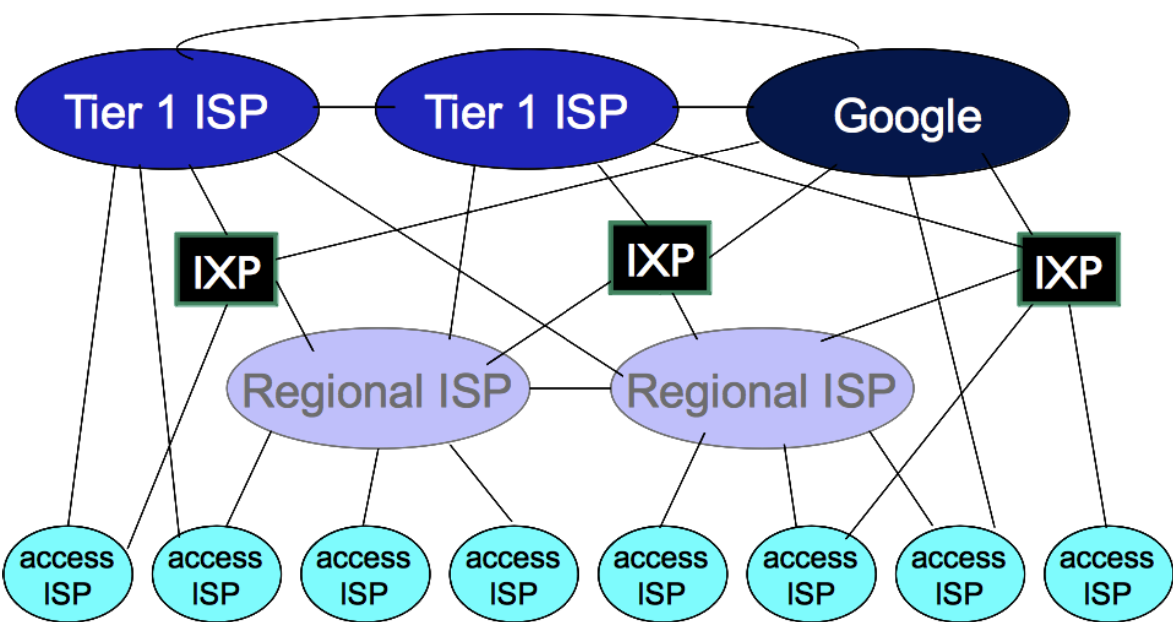
\includegraphics[width=0.45\linewidth]{res/ISPs1.png}
    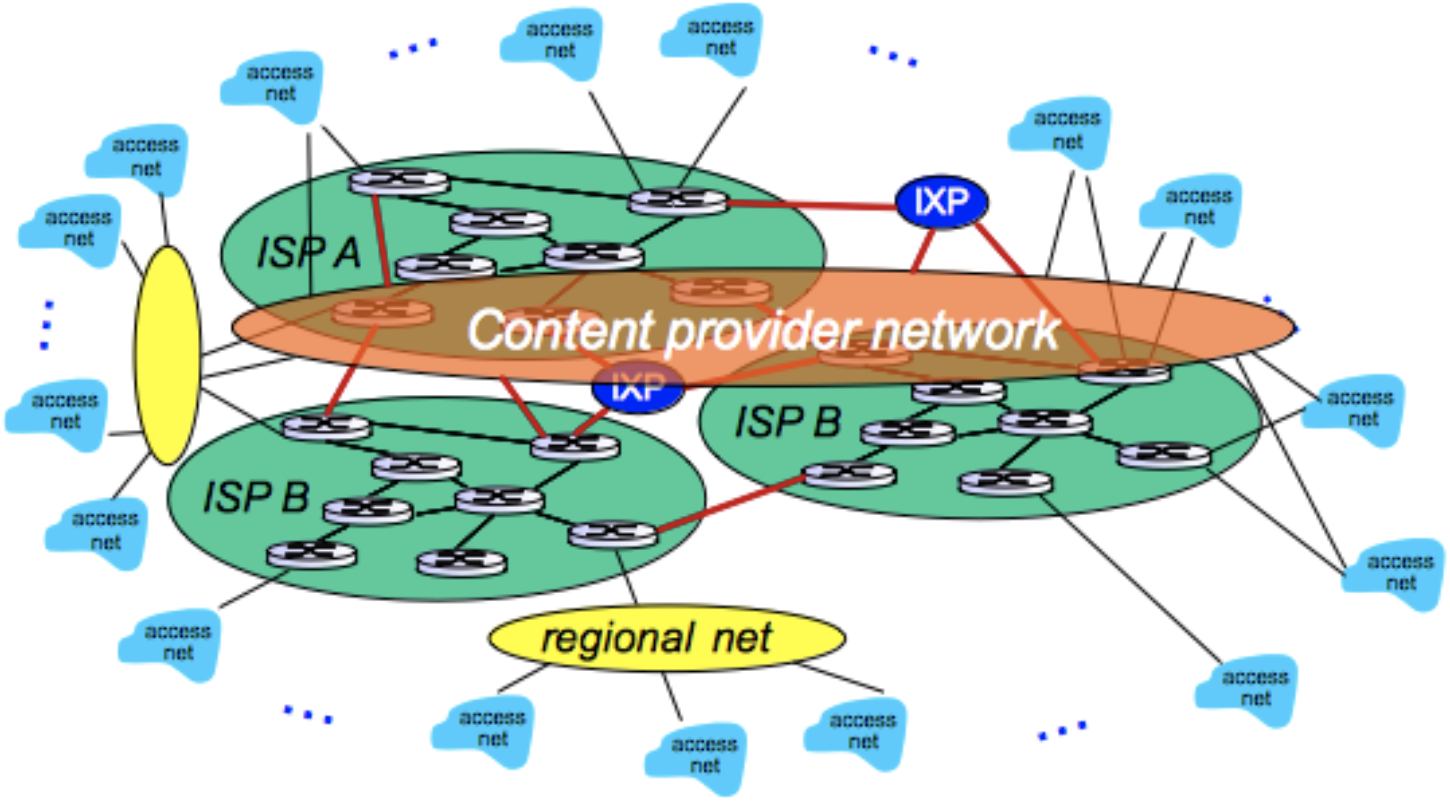
\includegraphics[width=0.45\linewidth]{res/ISPs2.png}
\end{figure}
\subsubsection{Delay, Loss, Throughput}
Abbiamo 4 fonti di packet delay:
\begin{itemize}
    \item $d_{proc}$, nodal processing: il nodo verifica errori e determina dove outputtare il packet 
    \item $d_{queue}$, queueing delay: tempo di attesa all'output per la trasmissione
    \item $d_{trans}$, transmission delay: dipendente dal link, quindi $L/R$
    \item $d_{prop}$, propagation delay: livello fisico del link, $l/v$ con $l$ lunghezza del link e $v$ velocità di propagazione nel mezzo 
\end{itemize}
Tramite un \textbf{traceroute} possiamo misurare il delay dalla fonte ai router attraverso il path. Per tutte le i, invia 3 pacchetti che raggiungeranno il router $i$ sul path, che li invierà indietro. 
\paragraph{Traffic intensity} Con traffic intensity, intendiamo la quantità $La/R$, con $L$ packet size, $a$ rateo di arrivo in queue, $R$ transmission rate. Questa quantità dovrebbe essere sempre $<1$, in quanto se fosse maggiore la queue si starebbe allungando.
\paragraph{Throughput} È il rateo a cui i bit vengono trasferiti tra sender e receiver. Distinguiamo tra istantaneo e medio. Il throughput più basso è sempre quello che comanda.
\subsubsection{Protocol Layers}
Le funzioni di rete sono strutturate a livelli: ogni livello $n$ comunica con l'altro livello $n$, con dati scambiati detti \textbf{Protocol Data Unit} (PDU). Il layer $n$ utilizza i servizi del layer $n-1$, e fornisce servizi ad $n+1$, con i dati di interfaccia detti \textbf{Service Data Unit} (SDU). La PDU è quindi formata da PCI (informazioni di controllo di protocollo) e SDU (il payload vero e proprio). Le entità a pari livello sono dette \textbf{peer entities}, operazioni tra peer entitites sono dette \textbf{procedure}. Il layering è una struttura esplicita che permette relazioni semplici, manutenzione semplice, update pure. 
L'architettura di rete (modello OSI) consiste in:
\begin{itemize}
    \item Application, Presentation, Session 
    \item Transport: process-process data transfer (TCP, UDP)
    \item Network: routing di datagrammi (IP)
    \item Link: data transfer tra elementi vicini 
    \item Physical: trasferimento fisico dei dati 
\end{itemize}
\subsubsection{Network Services}
Alcuni esempi di net services possono essere email, web, messaggistica, P2P, streaming\dots Per creare un network service scriviamo programmi che funzionino su sistemi differenti, comunichino in rete in modo end-to-end (il network core non c'entra nulla). Due processi in host differenti comunicano scambiandosi messaggi; un socket è l'endpoint di un link di comunicazione two-way tra due programmi funzionanti in rete. Il socket è collegato a un numero di porta in modo che il transport layer possa identificare l'applicazione corretta. 
\paragraph{Indirizzamento} Per ricevere messaggi, un processo deve avere un identificatore, basato su IP e porta. 
\subsubsection{TCP vs UDP} TCP fornisce trasporto affidabile, flow control, congestion control, ed è connection-oriented. Però non fornisce timing, minimo throughput garantito, sicurezza. UDP, invece, fornisce un data transfer inaffidabile. 
\subsection{HTTP}
Il \textbf{World Wide Web} è uno spazio di informazioni basato su internet, dove documenti e risorse sono identificati da indirizzi. Una \textbf{pagina web} è un documento HTML linkato ad altre pagine/risorse.
Gli \textbf{URI} (\textit{Uniform Resource Identifiers}) sono utilizzati in HTTP come mezzo identificativo delle risorse. 
\begin{center}
    \code{$schema:[//[user:password@]host[:port]][/]path[?query][\#fragment]$}
\end{center}
\textbf{HyperText Transfer Protocol} è un protocollo a livello applicativo, che adotta un modello client/server: uno \textbf{user agent} che inizia la connessione HTTP ed invia richieste, e un \textbf{origin server} che accetta le richieste e possiede le risorse. È inoltre utile definire altri tre termini:
\begin{itemize}
    \item \textbf{Local cache}: memoria locale (server o client)
    \item \textbf{Proxy}: applicazione intermediaria avente funzionalità server e client 
    \item \textbf{Gateway}: applicazione intermediaria che lavora per conto del server, senza renderlo noto ai client 
\end{itemize}
\subsubsection{Caratteristiche di HTTP}
\begin{itemize}
    \item \textbf{HTTP utilizza TCP}: il client inizia una connessione TCP (crea la socket) sul server, che accetta e comincia a scambiare messaggi, poi viene chiusa.
    \item \textbf{HTTP è stateless}: il server non mantiene informazioni riguardanti richieste passate 
\end{itemize}
Distinguiamo tra HTTP non-persistent, dove abbiamo un invio di risorsa alla volta, e persistent HTTP, dove più risorse vengono inviate attraverso una singola connessione TCP. Consideriamo il cosiddetto \textbf{Round Trip Time} (RTT): nella prima sono richiesti 2 RTT per risorsa (apertura connessione, invio risorsa), mentre la seconda lascia la connessione aperta, e quindi riduce il numero di RTT richieste. Inoltre, la seconda permette il \textbf{pipelining}, ossia l'invio di più richieste alla volta allo scopo di ridurre i tempi, senza attendere le risposte.
\begin{figure}[H]
    \centering
    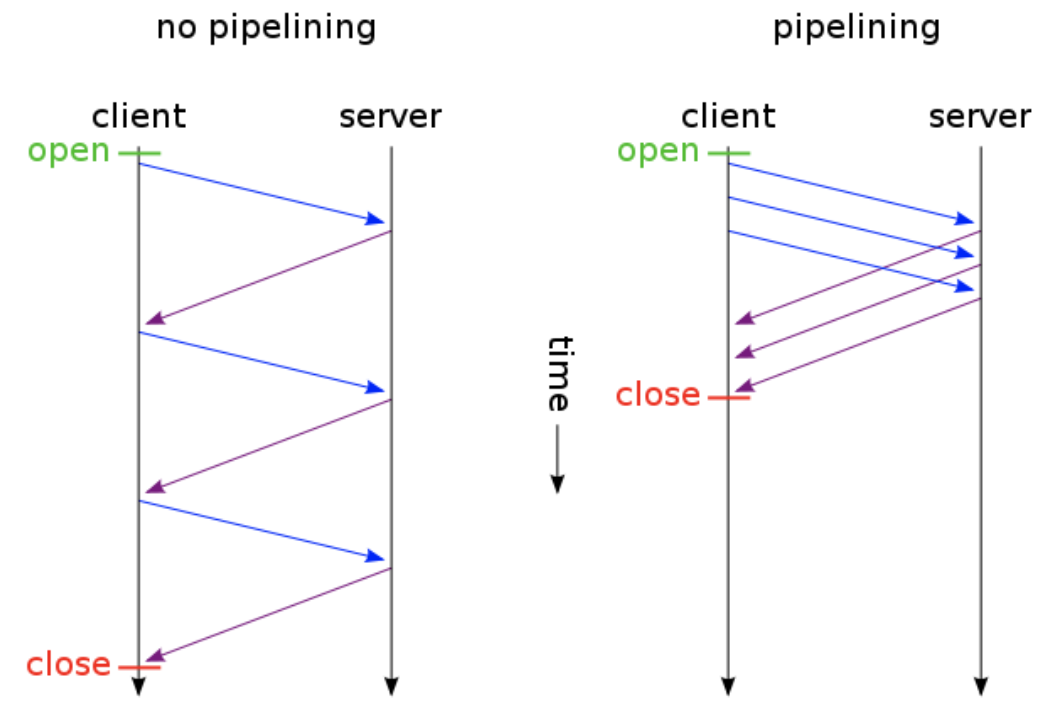
\includegraphics[width=0.6\linewidth]{res/pipelining.png}
\end{figure}
Un messaggio HTTP è formato da request/status line, header, body. Una request line è composta da \code{metodo target versioneHTTP}. Una status line è \code{versioneHTTP statusCode reasonPhrase}. Gli headers sono in formato MIME e specificano i metadati della richiesta come data, versione MIME, encoding, connessione, proxy/gateway, content-type, content-length, encoding, linguaggio, scadenza, data di modifica\dots Termina sempre con un carriage return (\code{\textbackslash r\textbackslash n}). 
\subsubsection{Metodi HTTP}
Prima di elencare i metodi, denotiamo due caratteristiche:
\begin{itemize}
    \item \textbf{Idempotenza}: significa che il metodo, chiamato più volte, restituirà sempre lo stesso risultato.
    \item \textbf{Safety}: significa che il metodo non modifica le risorse.
\end{itemize}
Procediamo elencando i metodi:
\begin{itemize}
    \item \textbf{GET}: \textit{safe ed idempotente.} Utilizzato per richiedere una risorsa, ottenuta nella risposta.
    \item \textbf{POST}: \textit{non safe, non idempotente.} Utilizzato per creare/aggiornare una risorsa. Chiamato ripetutamente, creerà più volte la risorsa.
    \item \textbf{PUT}: \textit{idempotente ma non safe.} Utilizzato per creare/aggiornare una risorsa.
    \item \textbf{DELETE}: \textit{idempotente ma non safe.} Elimina la risorsa specificata.
    \item \textbf{HEAD}: \textit{safe ed idempotente.} Come una GET ma restituisce solo l'header del messaggio.
\end{itemize}
Prima di procedere, distinguiamo le differenze tra POST e PUT: nella creazione di risorse, POST non specifica l'ID, mentre PUT si. Nell'update, POST permette di inviare la risorsa parzialmente (solo la parte da updatare), mentre PUT richiede la risorsa completa.
\subsubsection{Header delle richieste HTTP}
L'header contiene varie informazioni:
\begin{itemize}
    \item User-Agent: descrive il client che ha originato la richiesta
    \item Referer: URL della pagina che ha generato la richiesta 
    \item Host: dominio e porta a cui viene eseguita la richiesta
    \item From: indirizzo email del requester 
    \item Range: range della richiesta (utilizzato per riprendere i download)
    \item Accept, Accept-Charset, Accept-Encoding, Accept-Language: si spiega da solo; il client specifica cosa può accettare, il server decide il suo preferito
    \item If-Modified-Since, If-Unmodified-Since: permette di creare GET condizionali, ad esempio se ho una risorsa in cache e voglio verificare che sia aggiornata
    \item Authorization, Proxy Authorization 
\end{itemize}
\subsubsection{Messaggi di risposta HTTP}
La status line contiene un codice di stato:
\begin{itemize}
    \item 1xx - Informational: temporaneo mentre la richiesta viene eseguita
    \item 2xx - Successo: richiesta eseguita 
    \item 3xx - Redirection: il server ha ricevuto la richiesta ma sono necessarie altre azioni del client 
    \item 4xx - Client error: la richiesta è sbagliata
    \item 5xx - Server error: il server non è riuscito ad eseguire la richiesta 
\end{itemize}
Nell'header troviamo:
\begin{itemize}
    \item Server: stringa che descrive il server 
    \item WWW-Authenticate: contiene una challenge per il client; in caso di 401 unauthorized, il client utilizzerà la challenge per generare un codice di autorizzazione.
    \item Accept-Ranges: specifica il tipo di ranges accettabili (bytes/nulla)
\end{itemize}
\subsubsection{Cookies}
Molti siti utilizzano i cookies. Essi sono composti da 4 componenti: header line della prima risposta HTTP, header line nella prossima richiesta HTTP, file sull'host, DB sul backend del sito. 
\subsubsection{Proxy}
Il proxy è un'applicazione intermediaria che ha funzionalità server e client. Un \textbf{transparent proxy} non modifica la richiesta o risposta (es. HTTP tunneling), un \textbf{non-transparent proxy} modifica la richiesta/risposta per fornire servizi aggiuntivi.
Possiamo utilizzare un proxy server per soddisfare richieste senza coinvolgere il server originale: se la richiesta è nella cache, restituisce la risposta, altrimenti la inoltra. 
\subsection{Apache}
\textbf{Apache} nasce dal desiderio di migliorare httpd, il software server più utilizzato agli inizi di internet; è attualmente utilizzato per mantenere più del 50\% di internet. La sua architettura
 è formata da: 
 \begin{itemize}
     \item Moduli: compilati staticamente nel server o contenuti in una directory /modules o /libexec, caricata dinamicamente a runtime
    \item Apache httpd: implementa il ciclo di processamento delle richieste, composto da più fasi
    \item Multi-Processing Module: strato intermedio tra Apache e il sistema operativo, che gestisce i thread/processi
    \item Apache Portable Runtime: librerie che forniscono uno strato tra il sistema operativo e le utilities, in modo da poter essere portable
    \end{itemize}
Apache 2.0 utilizza un processo per connessione, I/O blocking. I Multi-Processing Modules bindano le porte della macchina e accettano richieste. 
\subsubsection{Configurazione}
La configurazione è eseguita tramite semplici file di testo, posizionati in varie directory e spesso divisi in più file e caricati tramite \textit{Include directives}. Una configurazione minimale richiede 5 directives:
\begin{enumerate}
    \item \code{User}: setta lo user ID con cui il server risponderà a richieste (utilizzare i permessi minimi)
    \item \code{Group}: setta il gruppo con cui il server risponderà a richieste (necessario avviare il server come root inizialmente)
    \item \code{ServerName}: setta lo schema delle richieste, hostname e porta. È in pratica l'URI.
    \item \code{DocumentRoot}: setta la directory di base delle richieste, a meno di specifiche di \textit{Alias.}
    \item \code{Listen}: setta la/le porta/e su cui accettare richieste
\end{enumerate}
In più, abbiamo:
\begin{itemize}
    \item \code{ErrorLog}: indica dove salvare il log degli errori
    \item \code{CustomLog}: indica un file dove salvare un log delle richieste, ed un filtro per decidere quali richieste loggare.
    \item \code{Include}: permette di includere altri file di configurazione
    \item \code{LoadModule}: linka una libreria/file oggetto e lo aggiunge ai moduli attivi.
    \item \code{IfModule}: permette di verificare se un modulo è installato ed eseguire directives di conseguenza.
\end{itemize}
Tramite \textbf{virtual hosting} possiamo hostare più siti sullo stesso server, distinguendoli in due possibili modi: tramite IP o nome. Con la seconda, non c'è necessità di IP multipli. 
Possiamo anche applicare delle configurazioni locali in determinate directory, e tramite le Options directives attivare/disattivare features, come: ExecCGI, FollowSymLinks, SymLinksIfOwnerMatch, Includes, IncludesNOEXEC, Indexes.
Inoltre, è possibile utilizzare i file \code{.htaccess} per definire cambiamenti alla configurazione in directories: inseriamo il file in una cartella e tutte le modifiche alla configurazione verranno eseguite lì e nelle subfolders. Tramite la \code{AllowOverride} della configurazione, decidiamo quali directives possono essere overridate dagli htaccess. Per migliorare le performance di Apache, il sistemista può modificare le opzioni di Apache: è però sconsigliabile usare spazio di swap (RAM virtuale). Infine, con la directive \code{ErrorDocument}, specifichiamo cosa fare quando si incorre in un errore HTTP specifico, con 4 possibilità: messaggio hardcoded di errore (default), messaggio custom, redirect interno, redirect esterno.
\subsubsection{Avvio di Apache}
Su \href{https://www.youtube.com/watch?v=dFUlAQZB9Ng}{sistemi Unix} httpd viene eseguito come daemon continuamente; se la directive Listen è sulla porta 80, è necessario avviare Apache come root perché è una porta speciale (poi verranno lanciati child processes). Lanciamo Apache con l'\code{apachectl} control script, che setta le variabili ENV necessarie e poi avvia httpd. Se l'avvio è succesful, il server viene detacchato dalla console (scusate). Si può usare apachectl per terminare Apache, o killare il daemon.
\subsection{HTML}
Il web è basato su tre risorse: gli URI, i protocolli, e HTML. \textbf{HTML} è un linguaggio universale che permette la creazione di documenti con formattazioni, contenuti, link, design. Nasce dalla mente di Tim Berners-Lee e conta attualmente 5 versioni major, la cui ultima è 5.2. Per promuovere l'interoperabilità, ogni documento HTML deve specificare il suo character set, formato da repertorio e code positions. Inoltre, va specificato l'encoding nell'header delle richieste HTTP. Distinguiamo tra 3 parti: una linea di versione HTML, un header, un corpo. Nell'header possiamo trovare varie tipologie di tag: \code{TITLE}, \code{BASE}, \code{LINK}, \code{SCRIPT}, \code{STYLE}, \code{META}. Nel corpo, possiamo trovare DIV (block-level) e SPAN (inline). Un heading descrive l'argomento della sezione che introduce (H1..H6 in base all'importanza). Abbiamo anche alcuni tag per il testo: \code{BR} va a capo, \code{P} delimita un paragrafo, \code{PRE} delimita un testo preformattato, \code{EM}, \code{STRONG}, \code{CITE}, \code{DFN}, \code{CODE}, \code{SAMP}, \code{KBD}, \code{VAR}, \code{ABBR}, \code{ACRONYM}, \code{BLOCKQUOTE}, \code{Q}, \code{SUB}, \code{SUP}. Possiamo creare liste: \code{UL} (\textit{Unordered List}), \code{OL}(\textit{Ordered List}), \code{DL}(\textit{Definition List}). Possiamo creare tabelle: \code{TABLE, TR, TD}. Possiamo spaziarle utilizzando \code{rowspan} e \code{colspan}, captionarle con \code{CAPTION}. Possiamo creare links con il tag \code{A}, avente attributi \code{href} e \code{target}(\_blank, \_self, \_parent, \_top). Dando ID agli elementi HTML possiamo cercarli tramite gli anchor link (\#riferimento). Con l'elemento \code{IMG} embeddiamo immagini definite nell'attributo \code{src}. Con \code{OBJECT} definiamo oggetti come risorse, applets, plugin. Con i frame possiamo generare views multiple; un frame ha head, frameset e body, con attributi rows e cols. Possiamo anche creare forms, che contengono contenuto, markup, controlli, labels e li inviano ad un'action (tramite GET o POST). In HTML5 sono stati inoltre definiti nuovi tag, semantici (header, footer, article, section), di controllo (numeri, date, orari, calendari, range), grafici (svg, canvas), multimediali (audio, video). Non sono più supportati i frames, sostituiti dagli iframes.
\subsection{CSS}
HTML non è nato per contenere tag di definizione di stile, ma piuttosto per mostrare dati. Quando cominciarono a venire aggiunti tag di stile ad HTML 3.2, come \code{font}, \code{color}, si capì che non poteva funzionare. Il World Wide Web Consortium (W3C) creò quindi \textbf{Cascading Style Sheets} (CSS). In HTML4, tutta la formattazione poté quindi essere definita separatamente dall'HTML, dando la possibilità di modificare l'intero sito con un solo file CSS. 
\subsubsection{Sintassi}
La sintassi consiste in un selettore, seguito da varie dichiarazioni:
\begin{center}
    \code{h1 \textbraceleft}
    \code{color:blue;}
    \code{font-size:12px;}
    \code{\textbraceright}
\end{center}
Il selector punta all'elemento HTML desiderato, mentre nel blocco di dichiarazione inseriamo una o più dichiarazioni separate da ;.
I selettori possono indicare una tipologia HTML, come \code{p}, una classe, come \code{.rowDiv}, un ID, come \code{\#title}. Possiamo includere CSS in tre modi:
\begin{itemize}
    \item Style sheet esterno: \code{<LINK rel="stylesheet" type="text/css" href="file.css">}
    \item Style sheet interno: \code{<STYLE> body\textbraceleft\textbraceright</STYLE>}
    \item Inline: \code{<H1 style="color:blue;">}
\end{itemize}
\subsubsection{Attributi notevoli}
Alcuni attributi importanti:
\begin{itemize}
    \item \textbf{Background}: background-color, background-image, background-repeat, background-attachment, background-position
    \item \textbf{Text}: color, text-align, text-decoration, text-transform, text-indent
    \item \textbf{Fonts}: permette di definire una font family (generica o specifica) con sistema fallback: le prova in ordine finché non trova la funzionante; è quindi meglio partire con specifica e terminare con generica. Oltre a font-family, abbiamo font-style (italic, oblique), font-size, font-weight
    \item \textbf{Links}: possiamo applicare ogni CSS property, ed in più abbiamo 4 selector speciali (A:link, A:visited, A:hover, A:active)
    \item \textbf{Lists}: possiamo settare i marker delle liste, o addirittura immagini come item markers con list-style-image 
    \item \textbf{Tables}: possiamo specificare i borders tramite la proprietà border, e anche width/height. Inoltre, anche text-align e vertical-align sono disponibili.
\end{itemize}

\subsubsection{Box model}
In CSS sfruttiamo il \textit{pattern} del box model: essenzialmente è ciò che wrappa un contenuto, che ci permette di aggiungere padding, bordi, margini. 
\begin{figure}[H]
    \centering
    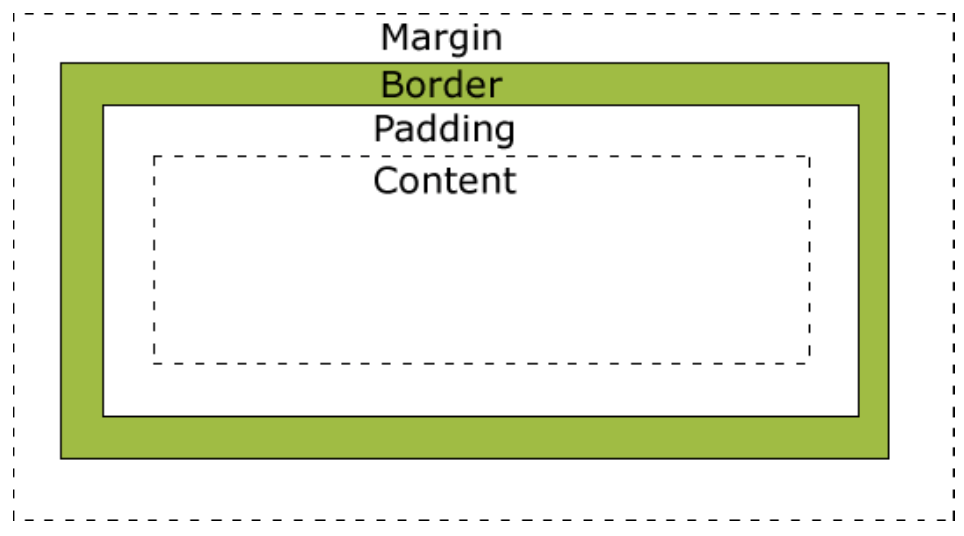
\includegraphics[width=0.6\linewidth]{res/boxmodel.png}
\end{figure}
\subsection{XML}
Sembrerà un linguaggio inutile e passato (perché lo è), ma nella sezione SOA ci sono ben due lezioni che si basano su sto schifo. \textit{Ocio.} XML sta per \textbf{eXtensible Markup Language} e serve per trasportare informazioni, non per presentarle (come HTML). I tag non sono definiti in uno standard, ma dall'utente. Possiamo, per esempio sfruttare XML per separare i dati variabili da HTML. 
\paragraph{Quando usare XML?} XML semplifica il salvataggio e la condivisione di dati, essendo un formato standard basato su testo. Semplifica i cambiamenti di piattaforma, essendo testo semplice. Tra i linguaggi scritti in XML, citiamo SVG, WSDL, RSS.
\subsubsection{Struttura}
Il documento XML inizia con il prologo, che definisce la versione XML. Comincia poi l'albero, che ha una root e delle leaves. I figli sullo stesso livello sono detti siblings (fratelli). Tutti i figli possono avere un contenuto e degli attributi. In XML è illegale omettere il tag di chiusura (tranne ovviamente nel prologo). I tag XML sono \textbf{case sensitive}. Gli attributi devono essere sempre tra virgolette. I commenti sono come in HTML: \code{<!-- Commentino -->}. XML non tronca gli spazi bianchi come HTML, e salva le nuove linee come \code{LF}. Bisogna stare attenti ad alcuni caratteri, come $<$, che vanno escapati con sequenze specifiche: \&gt;, \&amp, \&apos, \&quot;. Gli elementi XML devono seguire alcune regole di nomenclatura:
\begin{itemize}
    \item Case sensitivity
    \item Inizio con lettera o underscore
    \item Non si può iniziare con "XML"
    \item Possono contenere lettere, numeri, trattini, underscore, punti
    \item Non possono contenere spazi 
    \item Le lettere accentate non sono un problema (ma occhio ai software)
\end{itemize}
Gli attributi solitamente forniscono informazioni che non sono parte dei dati, ad esempio, se avessimo un contenuto file, l'attributo potrebbe essere il filetype. Alcuni problemi degli attributi:
\begin{itemize}
    \item Non possono contenere valori multipli
    \item Non possono contenere alberi 
    \item Non sono facilmente espansibili
\end{itemize}
Per evitare conflitti di nomi, possiamo utilizzare dei prefissi di namespace con l'attributo \textbf{xmlns}:
\begin{verbatim}
<h:table xmlns:h="http://www.w3.org/TR/html4/"> 
    <h:tr>
        <h:td>Apples</h:td>
        <h:td>Bananas</h:td>
    </h:tr>
</h:table>
\end{verbatim}
Dopo aver definito un namespace, tutti i contenuti con quel prefisso verranno collegati al namespace. Definire un namespace di default è utile: ci evita di utilizzare prefissi in tutti i children. 
Possiamo utilizzare anche caratteri internazionali: è però importante specificare l'encoding nel prolog. 
\subsubsection{Validità e document types}
Un documento XML corretto è detto \textit{ben formato}. Un documento XML valido deve essere compatibile con una \textbf{document type definition}. Ne abbiamo due diverse tipologie: DTD (\textit{Document Type Definition}) e XML Schema (\textit{basata su XML}). Usiamo questi document type per vari scopi: decidere standard, verificare dati dall'esterno, verificare dati nostri. XML non lo richiede per forza, ma in ambienti di produzione ci vuole. Lo scopo di un DTD è definire la struttura, con una lista di elementi validi. Possiamo anche usarlo per definire caratteri speciali e stringhe di caratteri. L'\textbf{XML Schema} è un'alternativa basata su XML a DTD.

\subsection{JSON}
\textit{Finalmente.} JSON è il cugino che ce l'ha fatta di XML. Sta per \textbf{JavaScript Object Notation}, ed è come XML una sintassi per salvare e scambiare dati, più leggera e semplice di XML. Dal momento che JSON è proprio il modo di definire oggetti in JavaScript, non necessita di parser. Similarità con XML: self-describing, gerarchico, portable, fetchabile con una XMLHttpRequest. Differenze con XML: niente tag di chiusura, più breve, più veloce, presenza di arrays. La sintassi di JSON è derivata da JS: i dati sono accoppiati nome/valore, separati da virgole, oggetti delimitati da \textbraceleft\textbraceright, arrays delimitati da $[]$. Un valore JSON può essere un numero, stringa, boolean, array, oggetto, null.
\subsection{Search Engines}
L'\textbf{information retrieval} è parte della computer science che studia il recupero di informazioni da una collezione di documenti, soddisfando le necessità dell'utente, solitamente definite in linguaggio naturale. 
La \textbf{web search} è molto simile, con alcune differenze: links tra web pages, collezionare documenti è molto più difficile, il numero di utenti è grande, lo spam è un problema. La struttura di un web search engine è composta da un downloader, un crawler, un indexer\dots Abbiamo eterogeneità multiple: utenti, linguaggi, document types, queries (informational, navigational, transactional, connectivity). Un crawler feeda continuamente l'indexer con informazioni nuove o aggiornate. Distinguiamo inoltre tra surface web, indexato, e deep web (da non confondere con darkweb) ossia la parte di internet non indexata, composta da pagine dinamiche, contenuti privati, script, formati particolari. 
\subsubsection{Web Graph}
Possiamo vedere le pagine, linkate tra loro, come un grafico di pagine collegate tra in-links e out-links. La distribuzione dei links non è randomica ma segue una \textit{power law}: il numero di pagine con k \textit{in-links} è proporzionale a $k^{-2.1}$. Alcuni studi hanno mostrato che il web graph ha \textit{bowtie shape}. 
Un crawler consiste in una queue di URI da visitare, un metodo per ottenere i dati, un parser che estragga i link, una connessione all'indexer. Il crawler dev'essere highly scalable: abbiamo 60mld di pagine sul web. Dobbiamo inoltre tenere conto di altri problemi: spam, duplicati, spider traps, distribuzione, latenza, banda, profondità, desideri dell'owner. In quanto owner possiamo escludere alcune risorse dall'accesso dei robots, tramite il file robots.txt. Per l'indexing, sfruttiamo la link analysis: i link sono raccomandazioni, gli anchor texts descrizioni del documento. 
\subsubsection{PageRank}
PageRank è l'algoritmo di Larry Page (il signor Google) sviluppato a Stanford. È un algoritmo di link analysis che produce un ranking non dipendente dalle queries. È eseguito periodicamente dall'indexer. L'algoritmo si basa sulla probabilità che un utente random clicki su un link che porti alla pagina da un'altra, calcolata ricorsivamente sulla probabilità della pagina attuale e via andare\dots PageRank è usato ancora oggi (in parte), soprattutto in formato topic-sensitive: una pagina su un topic specifico può non essere utile globalmente ma essere importante per il topic stesso. 
\subsubsection{HITS}
HITS è un altro algoritmo. Cominciamo col distinguere due tipi di pagine web: authorities (fonti autoritarie sull'argomento), hubs (puntatori all'authority). C'è una relazione di reinforcement: hub di qualità puntano ad authorities di qualità. Seguiamo due fasi:
\begin{enumerate}
    \item \textbf{Sampling phase}: le parole della query vanno a costruire un root set di pagine, che viene espanso a un base set, aggiungendo tutte le pagine linkate dal root set
    \item \textbf{Weight-propagation phase}: ogni pagina riceve un authority-weight $a_p$ e un hub-weight $h_p$ pari a 1. A questo punto, $a_p$ è la somma degli hub weights che puntano alla pagina, mentre $h_p$ è la somma degli authority weights delle pagine linkate da p. Poi, applichiamo una normalizzazione finché i weights non convergono. 
\end{enumerate} 
A volte HITS tende a generalizzare o a deviare dal topic, soprattutto quando gli hubs coprono più topic; una soluzione potrebbe essere comparare le parole della query con quelle che circondano il link, o frammentare un grande hub in hublets minori, ed ignorare quelli unrelated. 
\subsubsection{HITS vs PageRank}
PageRank può essere precomputed, mentre HITS deve essere computato a query time. Abbiamo poi scelte diverse riguardanti il modello formale.

\section{JavaScript}
\subsection{Basics}
JavaScript è il linguaggio di programmazione che permette di programmare il comportamento delle pagine web. Seguendo il pattern MVC, abbiamo che il model è gestito da XML/JSON, la view da HTML+CSS, il controller da JavaScript. JavaScript non è Java e non è un linguaggio di scripting. ECMAScript è la standardizzazione ufficiale del linguaggio. Il core di JS definisce un'API minimale, ma è l'environment ad avere le responsabilità maggiori: il browser, Rhino o Node. 
Possiamo embeddare JS in HTML tramite: inline (tag \code{<script>}), esterno (sempre tag \code{<script>} con \code{src}), in un event handler come l'onclick, in un URL che utilizza il protocollo \code{javascript:}. Una filosofia detta \textbf{unobstrusive JavaScript} sottolinea che contenuto (HTML) e comportamento (JS) devono essere il più separati possibile. JS non ha metodi di print definiti, ma usiamo \code{window.alert()}, \code{document.write()}, \code{innerHTML}, \code{console.log()}. Gli statement sono separati da ;, e composti da valori, operatori, espressioni, keywords, commenti. Distinguiamo tra valori fissi (\textbf{literals}) e variabili (\textbf{variables}). Utilizziamo la keyword \code{var} per definire variabili, che in JS sono \textbf{untyped}. Essendo untyped abbiamo possibilità di confusione; JS interpreta le operazioni da sinistra a destra. 
\begin{figure}[H]
    \centering
    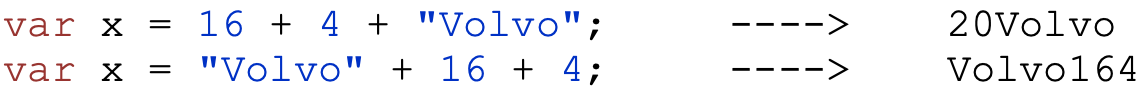
\includegraphics[width=0.4\linewidth]{res/JSconfusion.png}
\end{figure}
Abbiamo i soliti operatori; la concatenazione di stringhe è fatta con \code{+}. Esiste l'operatore condizionale \code{ ? : }. I commenti sono fatti con \code{//} e \code{/* */}. Gli identifiers possono iniziare con lettere, underscore o dollaro e contenere lettere, numeri, underscores, dollari. Gli identifiers sono case sensitive. Le funzioni sono definite dalla keyword \code{function} seguita da nome e argomenti. Le variabili possono anche contenere oggetti, definiti con la forma classica di JS. Inoltre, gli oggetti possono contenere funzioni (questo è importante) come se fossero semplici attributi. Possiamo creare oggetti in tre modi: con l'object literal (come JSON), con la keyword new \code{Object ()} e poi settando attributi, o con una funzione costruttrice. Gli oggetti creati con i primi due metodi ereditano da un prototipo detto \code{Object.prototype}, che è in cima alla scala gerarchica. JS ha costruttori per gli oggetti nativi, come Object, String, Number, Boolean, Array, RegExp, Function e Date, ma è meglio utilizzare i literals, come \textbraceleft\textbraceright, "", 0, false, $[]$, $/()/$, function$(){};$. Gli oggetti sono indirizzati per reference, non valore, quindi la copia non è fattibile con $=$. Possiamo aggiungere attributi ad un oggetto semplicemente assegnandoli, ed eliminarli con la keyword \code{delete}. Tramite la proprietà prototype, possiamo modificare prototipi già definiti. 
\begin{figure}[H]
    \centering
    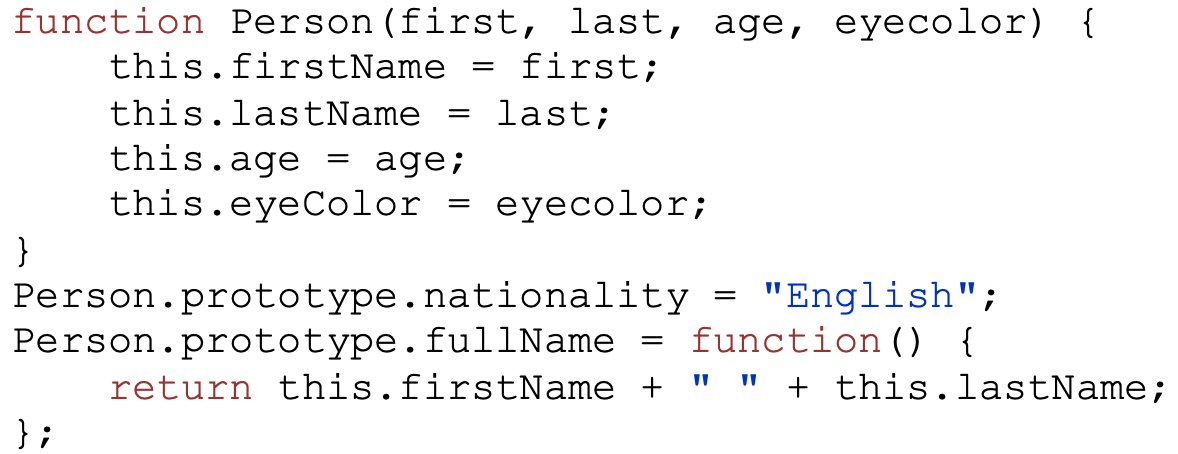
\includegraphics[width=0.4\linewidth]{res/prototype.png}
\end{figure}
Possiamo loopare tra tutte le proprietà di un oggetto usando \code{for..in}.
La sintassi \code{with (object)${}$} utilizza object come prefisso di tutti gli statement enclosati. Con ECMAScript6 sono state introdotte le classi OOP, con eredità. Gli arrays sono oggetti speciali con indici numerici e non testuali, che hanno dei metodi built-in comodi come \code{length}, \code{sort()}, \code{pop()}, \code{push()}. La sort lavora però su stringhe, quindi ad esempio 25 è più grande di 100. Possiamo comunque fornire come argomento una compare function. 
\subsection{Client-side JS}
L'oggetto window è l'entry point principale di tutte le feature di JS client-side. JavaScript è più puntato sulle web applications che sui web documents: i secondi funzionano con JS disattivato, le prime no. Quando un HTML parser incontra uno script, lo esegue di default. Solo gli script sincroni possono usare \code{document.write()} per inserire testo nell'input stream. Il tag script può avere attributi \code{defer} e \code{async}: il primo lo esegue a fine caricamento, il secondo lo esegue al più presto ma senza bloccare il parsing. Il core di JS non contiene meccanismi di threading, quindi due event handlers non gireranno mai allo stesso tempo; l'esecuzione single-threaded significa che i browser devono smettere di rispondere agli input quando gli script vengono eseguiti. Se c'è molta computazione, sarebbe meglio lasciar caricare il documento prima. Questa la timeline degli eventi:
\begin{enumerate}
    \item Il browser crea un oggetto document e comincia a parsare la web page, aggiungendo gli elementi e i text nodes. \code{document.readyState} è ora "loading"
    \item Quando l'HTML parser incontra degli elementi \code{<script>} senza async o defer, li aggiunge al documento e li esegue. 
    \item Quando l'HTML parser incontra degli script async comincia a scaricare lo script e continua a parsare. Lo script verrà eseguito appena scaricato.
    \item Quando il documento è parsato, \code{document.readyState} è "interactive"
    \item Ogni script con l'attributo defer viene eseguito nell'ordine di lettura. Questi hanno accesso alla document tree e non devono usare \code{document.write()}. 
    \item Il browser lancia un evento \code{DOMContentLoaded} sull'oggetto document. Questo segna la transizione dalla fase sincrona di esecuzione alla fase asincrona event-driven. 
    \item Il documento è parsed, ma potrebbero ancora mancare risorse come le immagini. Quando è tutto pronto, \code{document.readyState} passa a "complete"
\end{enumerate}
JS non fornisce alcun metodo per scrivere o eliminare file sul computer, ma può ottenere un FileSystem privato. 
\subsubsection{Same Origin Policy}
La same origin policy indica che uno script può leggere solo le proprietà di finestre e documenti che hanno la stessa origine (protocollo, host, porta) del documento che contiene lo script. La policy è applicata alle richieste HTTP fatte con l'oggetto XMLHttpRequest, che permette al JS client-side di fare richieste HTTP al server da dove ha caricato il documento, ma non ad altri server. Per richieste cross-origin bisogna attivare \textit{Cross-Origin Resource Sharing}. 
\subsubsection{L'oggetto window}
L'oggetto \textbf{window} è l'oggetto globale per il client-side JS, le cui proprietà sono collegate a timers, location/navigation, history, browser informations, dialogs, document elements, comunicazione cross-window. 
\paragraph{Timers} I \textbf{timers} vengono settati con \code{setTimeout} che esegue una funzione dopo un numero definito di ms, e \code{setInterval}, che fa la stessa cosa ciclicamente ad intervalli.
\paragraph{Location e navigation} La proprietà \code{location} dell'oggetto window si riferisce ad un oggetto location, che rappresenta l'URL corrente e i metodi per far caricare alla window un nuovo documento. La proprietà \code{href} dell'oggetto location è una stringa contenente l'URL, altre proprietà sono protocol, host, hostname, port, pathname, search, hash. L'hash ritorna l'anchor link, mentre search le query delimitate da ?. Il metodo assign della location carica un nuovo URL, replace lo fa rimuovendo la pagina corrente dall'history, reload aggiorna. 
\paragraph{History} La proprietà \code{history} della window contiene la cronologia. Ha proprietà length, metodi \code{back()} e \code{forward()}, \code{go(n)} che va avanti o indietro di n passi
\paragraph{Navigator} La proprietà \code{navigator} contiene informazioni sul browser. L'utilizzo di queste informazioni è sconsigliato: è meglio utilizzare il feature testing. Tra le proprietà citiamo appName, appVersion, userAgent, platform. Abbiamo poi alcune proprietà non-standard: onLine, geolocation, javaEnabled(), cookieEnabled.
\paragraph{Screen} La proprietà \code{screen} fornisce informazioni sulle dimensioni e colori del display: width, height, availWidth, availHeight (escludono menubar ecc.), colorDepth. 
\paragraph{Dialogs} L'oggetto window fornisce tre metodi per generare dialogs: alert(), confirm(), prompt().
\paragraph{Elementi HTML} Ogni elemento del documento HTML avente un id diventa proprietà di window, contenendo l'oggetto HTMLElement. È però raccomandato utilizzare \code{document.getElementById()}. 
\paragraph{Multiple windows} La comunicazione tra windows è possibile solo tra finestre same-origin. Il metodo \code{open()} apre una nuova finestra e ritorna l'oggetto relativo, prendendo 4 argomenti: URL, nome, attributi size/feature, boolean che indica se creare un nuovo record nell'history. Il metodo \code{close()} chiude la finestra indicata. Possiamo anche accedere agli oggetti window degli iframe tramite \code{iframe.contentWindow} e al document tramite \code{iframe.contentDocument}. 
\subsubsection{Scripting di documenti}
Il DOM, \textbf{Document Object Model} è lo standard W3C per accedere ai documenti, separato in Core, XML, HTML. Quest'ultimo è uno standard e interfaccia di programmazione per HTML, definendo: gli elementi HTML come elementi, le proprietà, i metodi, gli eventi. Insomma: \textbf{l'HTML DOM è uno standard per come ottenere, modificare, aggiungere o eliminare elementi HTML.}
Per ottenere un elemento HTML il modo più semplice è usare \code{document.getElementById()}, per il contenuto poi usiamo \code{innerHTML}. Possiamo, inoltre, modificare gli attributi con \code{element.attribute}, e lo stile \code{element.style.property}. Possiamo aggiungere/rimuovere elementi al documento con \code{document.createElement()}, \code{document.removeChild()}, \code{document.appendChild()}, \code{document.replaceChild()}, \code{document.write(text)}, o settare event handlers con \code{document.getElementById(id).onclick = function $(){}$}. Altri modi di ottenere elementi sono getElementsByTagName e getElementsByClass, che ritornano liste (non array: sono navigabili allo stesso modo ma mancano alcuni metodi). L'HTML DOM ha una struttura ad albero, in cui gli elementi HTML sono nodi, aventi attributi \code{nodeName}, \code{nodeValue}, \code{nodeType}.
\subsection{Client side - AJAX}
Gli eventi HTML sono cose che accadono agli elementi HTML, a cui JS può reagire. Gli elementi HTML possono avere un attributo onclick a cui associare una funzione JS. Oltre ad onclick, abbiamo: onchange, onmouseover, onmouseout, onkeydown, onload\dots Gli event handler possono essere utilizzati per gestire gli input utente. L'HTML DOM permette di assegnare event handler agli elementi HTML. 
\paragraph{onload e onunload} Vengono triggerati quando l'utente entra o lascia la pagina, sono utilizzabili per controllare il browser, o gestire i cookies.
\paragraph{onchange} Utilizzato spesso per la validazione dei field.
\paragraph{onmouseover e onmouseout} Triggerano una funzione quando l'utente sposta il mouse sull'elemento. 
\paragraph{onmousedown, onmouseup, onclick} Si spiegano da soli: il primo è il down, poi up, infine click. 

Utilizziamo il metodo \code{element.addEventListener(event, function, useCapture)} per aggiungere un event listener. Distinguiamo tra bubbling (primo trigger è il più interno) e capturing (primo trigger è il contenitore) come metodi di trigger. Utilizzando \code{addEventListener} possiamo aggiungere più event handlers a uno stesso evento. 
\subsubsection{AJAX}
AJAX significa \textbf{Asynchronous JavaScript and XML}, ed è una tecnica per creare pagine web veloci e dinamiche. AJAX permette di aggiornare le webpages in modo asincrono, scambiando dati con il server e modificando il contenuto senza ricaricare tutta la pagina. Il punto chiave di AJAX è l'oggetto \code{XMLHttpRequest}, che permette di fare richieste HTTP. Bisogna verificare se è supportato, altrimenti usare un ActiveXObject (\textit{Microsoft vaffanculo}). Apriamo la richiesta tramite \code{open(method, url, async)} e la inviamo tramite \code{send()} per GET e \code{send(string)} per POST. Per evitare di farci ritornare dati cachati, aggiungiamo alla GET una query casuale. Per aggiungere headers a una POST, utilizziamo \code{setRequestHeader(header, value)}. Bisogna stare attenti alla same-origin policy. Per ottenere la risposta, utilizziamo l'attributo \code{responseText} o \code{responseXML} dell'oggetto richiesta. Come il document, la request ha un attributo \code{readyState} (0..4), un relativo evento \code{onreadystatechange} e un attributo status che contiene lo status HTTP. Quando readyState è 4 e status 200, è andato tutto bene. Potremmo quindi aggiungere una callback all'onreadystatechange, verificando queste due condizioni prima.

\subsubsection{jQuery}
\textbf{jQuery} è una leggera libreria "\textit{write less, do more}" che rende più semplice il JS. Abbiamo due versioni, una di produzione minified, difficilmente leggibile, e una di sviluppo. Per utilizzare jQuery lo referenziamo nell'head del documento, hostandolo sul server o caricandolo da un CDN. La sintassi di jQuery permette di selezionare elementi HTML semplicemente: \$$($selettore$)$. Per evitare di eseguire codice jQuery prima del corretto caricamento della pagina, mettiamo il codice dentro un document ready event. In jQuery, la maggior parte dei DOM events hanno un metodo jQuery corrispondente, per esempio \code{\$("p").click(function$(){}$)}. jQuery permette anche di definire eventi custom, firabili con \code{trigger(nome, datiOpzionali)}, e handlabili con \code{.on("evento", function$(){}$)}. 
\subsubsection{Animazioni con jQuery}
jQuery permette anche di implementare animazioni: un esempio sono i metodi \code{hide(speed, callback)} e \code{show(speed, callback)}. Speed può essere "slow", "fast", o un valore di millisecondi. Callback viene invece eseguito al termine dell'animazione. Il metodo \code{toggle()} alterna tra show e hide. Abbiamo anche dei metodi di fade: \code{fadeIn(s, c)}, \code{fadeOut(s, c)}, \code{fadeToggle(s, c)}, \code{fadeTo(s, opacity, callback)}. Possiamo anche slidare elementi: \code{slideDown(s, c)}, \code{slideUp(s, c)}, \code{slideToggle(s, c)}. Grazie al metodo \code{animate(\textbraceleft parametri\textbraceright, s, c)} possiamo creare animazioni custom modificando proprietà CSS. Di default, jQuery lavora per queue sulle animazioni: le fa una alla volta.
\subsubsection{Manipolazione del DOM con jQuery}
jQuery permette anche di \textbf{manipolare il DOM} tramite 4 metodi che settano o leggono: \code{text()}, \code{html()}, \code{val()}, \code{attr()}. Abbiamo metodi per aggiungere contenuto: \code{append()}, \code{prepend()}, \code{after()}, \code{before()}. Metodi per rimuovere contenuto: \code{remove()} (filtrabile), \code{empty()}. Possiamo modificare il css: \code{addClass()}, \code{removeClass()}, \code{toggleClass()}, \code{css()}. Questo non è tutto: ci sono anche metodi per modificare dimensioni, navigare gli elementi, funzionalità AJAX (ad esempio, richieste GET con \code{\$.get(url, callback))}.
\subsubsection{Client-side storage}
Le web apps possono utilizzare API del browser per salvare dati sul computer. I dati salvati possono essere visualizzati solo da pagine dello stesso sito. Abbiamo più modi di salvare roba: WebStorage API, Cookies, Filesystem API\dots
\paragraph{Web Storage} L'API Web Storage fornisce due oggetti: \code{window.localStorage} (senza scadenza) e \code{window.sessionStorage} (eliminata con la chiusura della tab). Prima di utilizzarle è bene verificare la disponibilità della feature. 
\subsubsection{Scripted graphics}
Generare grafiche complesse nel browser è molto meglio: rimuove il carico dal server per affidarlo al computer, risparmiando in banda, CPU, RAM\dots Inoltre è consistent con le moderne architetture applicative. In HTML5 è stato introdotto l'elemento \code{<canvas>} che ha lo scopo di ospitare grafiche generate da JS. Deve ovviamente avere un ID per essere trovato da JS. Tramite \code{canvas.getContext()} otteniamo l'oggetto context, che contiene metodi per disegnare sul canvas, come \code{moveTo()}, \code{lineTo()}, \code{stroke()}, \code{beginPath()}, \code{arc(x, y, r, start, stop)}. Possiamo riempire anche con gradient: \code{createLinearGradient(x, y, x1, y1)}, \code{createRadialGradient(x, y, r, x1, y1, r1)} da riempire poi con \code{addColorStop()}. Possiamo scrivere nel canvas con le proprietà: \code{font}, \code{fillText(text, x, y)}, \code{strokeText(text,x , y)}, \code{fillStyle}, \code{textAlign}. Possiamo inserire immagini tramite \code{drawImage(img, x, y)}, opzionalmente con width e height o addirittura clippando l'immagine. 
\subsubsection{Frameworks importanti}
Elenchiamo ora alcuni framework importanti.
\paragraph{AngularJS} Citato come Model-View-Whatever, velocizza la programmazione, il testing, il data-binding.
\paragraph{Angular} Ha feature che permettono di creare prodotti vari, da web a desktop a mobile.
\paragraph{React} Creato ed utilizzato da Facebook, è molto efficiente con applicazioni ad alto traffico. È più impegnativo da imparare, ma diretto e semplice. 
\paragraph{Ember} Ottimo framework utilizzato da Chipotle, Kickstarter, LinkedIn, Netflix\dots
\paragraph{Vue} Introdotto nel 2016, cerca di unire il meglio di Ember, React, Angular in un pacchetto veloce e semplice. Molto utile per single page applications. 
\paragraph{Meteor} Permette sviluppo rapido e semplice di applicazioni end-to-end performanti. Citiamo inoltre alcuni IDE: WebStorm, Atom, VSCode (spacca), Brackets.
\subsection{Server side - NodeJS}
\textbf{Node} è una piattaforma costruita sul Chrome JavaScript runtime che fornisce un'API asincrona con I/O non-blocking che lo rende leggero ed efficiente. Il programma può richiedere una risorsa e continuare con il suo lavoro, poi una callback gestisce il risultato. Il giochino è lo stesso delle richieste HTTP su jQuery, semplicemente ora accediamo a un filesystem e non ad una risorsa remota. Node è designed per \textbf{data-intensive real-time}(DIRT) applications. È creato per essere responsive e per avere consistenza tra browser e server, reimplementando oggetti comuni come la Timer API e la Console API, aggiungendo un core set di moduli per network e file I/O: HTTP, POSIX (filesystem), DB\dots

Per rendere una pagina disponibile, ad esempio, ci basterà fare:
\begin{verbatim}
var http = require('http');
http.createServer(function (req, res) { res.writeHead(200, {'Content-Type': 'image/png'});
fs.createReadStream('./image.png').pipe(res);
}).listen(3000);
console.log('Server running at http://127.0.0.1:3000/');
\end{verbatim}
I dati sono letti dal file tramite uno stream, ed inviati al client (.pipe)
\subsubsection{Modularità}
È più facile navigare nel codice se è organizzato con directory e file separati. Il sistema di moduli di Node fornisce un meccanismo potente per organizzare il codice. I moduli ci permettono di selezionare quali funzioni e variabili del file incluso sono esposte all'applicazione tramite \code{exports}. \textbf{Node Package Manager} (npm) è una collezione online di moduli node. I moduli possono essere singoli file o directories; se è una directory, il file principale sarà index.js, a meno che non specifichiamo diversamente nel package.json. Per utilizzare il metodo, sfruttiamo la funzione \code{require} di Node, che prende un path come argomento. Require è una delle poche operazioni I/O sincrone di Node. 
\subsubsection{Programmazione asincrona}
Le \textbf{callbacks} definiscono la logica da eseguire al completamento di un'operazione. Gli event emitters firano eventi. Una callback è una funzione, passata come argomento ad una funzione asincrona, che descrive cosa fare dopo. Una caratteristica importante è che la maggior parte dei moduli di Node usano callbacks con due argomenti: err e res, il primo riempito solo in caso di errore. Gli \textbf{event emitters} firano gli eventi; molti componenti di Node, come i server HTTP o TCP e gli stream, sono implementati come event emitters, customizzabili con \code{channel.emit()}. 
\subsubsection{Sequenziare logiche asincrone}
Durante l'esecuzione di un programma asincrono, ci sono alcune task che possono accadere in ogni momento, mentre altre devono accadere solo prima o dopo altre. Il concetto di sequenziare gruppi di task asincrone è detto \textbf{flow control}, di cui distinguiamo due tipi: serial e parallel. 
\paragraph{Serial} Per implementare il flow control seriale, creiamo un array di tasks e lo attraversiamo una alla volta, grazie a un metodo \code{next(err, result)}, che chiameremo in fondo ad ogni funzione, e che shifta l'array ogni volta.  
\paragraph{Parallel} Anche qui, aggiungiamo le funzioni a un array dinamicamente, ad esempio scorrendo un albero di file, poi le facciamo partire in parallelo.
\subsubsection{Node e MySQL}
Possiamo utilizzare MySQL con Node installando il modulo corretto da npm. Poi, basta creare un oggetto connection da cui possiamo chiamare il metodo \code{connection.query(query, callback(err, rows, fields))}, che contiene le rows di risposta, scorribili con un for. Questa funzione query ha anche degli eventi 'error', 'fields', 'result', triggerati ad ogni risultato. Possiamo pausare la query per eseguire operazioni prima di proseguire coi risultati, tramite \code{connection.pause()} e \code{connection.resume()}. Connection ha inoltre un evento 'close', triggerato quando la connessione si chiude, volutamente o no. Possiamo controllare se 'err' è istanziato nella callback, in modo da catchare eventuali errori.
\section{Service Oriented Architectures}
La \textbf{Service-Oriented Architecture} è lo stile architetturale prevalente nei correnti middleware per sistemi informativi distribuiti.
L'obiettivo principale è permettere ad agenti debolmente coupled e software di cooperare. Un servizio è una work unit svolta da un provider, per ottenere un risultato richiesto da un consumer.
\paragraph{Servizio} Il servizio è una procedura, metodo o oggetto con interfaccia pubblica e stabile, invocabile da un client. Può essere considerato come la caratterizzazione astratta e incapsulamento dell'interfaccia di un contenuto/risorsa specifico.
\paragraph{Service Interface} Una \textbf{service interface} è definita in termini di \textbf{protocollo utilizzato} per interagire, \textbf{formato} dei dati scambiati, \textbf{comportamento atteso} dopo lo scambio di alcuni messaggi.
\paragraph{Ciclo di vita di un servizio} Un servizio ha 3 fasi di vita:
\begin{enumerate}
    \item \textbf{Creazione}: il servizio viene pubblicato in una directory o con advertisements
    \item \textbf{Procurement}: il provider e il consumer stabiliscono un service provision contract, tramite discovery e negotiation
    \item \textbf{Enactment}: il servizio è utilizzato
\end{enumerate}
\paragraph{Ruoli} La SOA è basata sull'interazione tra 3 ruoli: provider, registry, consumer.
\paragraph{Quality of Service} La stessa service interface può corrispondere a diverse implementazioni, con provider differenti e QoS diverse. La QoS è collegata ad aspetti non funzionali, tra cui performance, disponibilità, robustezza, autorizzazioni necessarie, costi. Provider e consumer devono stabilire un Service Level Agreement (SLA), che è un agreement di QoS. 
\subsection{XML-based Services}
Un XML-based service è un servizio implementato al web application layer, basato su un set di tecnologie XML-based. Nella maggior parte delle specifiche standard, i servizi XML-based sono detti \textbf{Web Services}.
La definizione formale vuole che: \say{Un web service è un componente software progettato per supportare interazione macchina a macchina in rete. Ha un'interfaccia definita in un formato processabile da macchine (WSDL). Altri servizi interagiscono in una maniera decisa dalla descrizione, tramite messaggi SOAP, tipicamente convogliati tramite HTTP con serializzazione XML.}
Insomma: se un componente software ha un'interfaccia descritta in WSDL ed interagisce con un client scambiando messaggi SOAP, è un web service. I web services permettono alle applicazioni di cooperare attraverso il web, in modo distribuito, platform-independent, programming language independent.
Quali sono le caratteristiche uniche dei web services?
\begin{itemize}
    \item Basato su XML
    \item Loosely-coupled: un consumer non è strettamente legato allo specifico web service 
    \item Coarse-grained: un pezzo di business logic 
    \item Permette composizione al volo di nuove funzionalità, composizione, decomposizione, distribuzione su larga scala.
\end{itemize}
3 standard definiscono gli elementi critici dei web services: \textbf{Simple Object Access Protocol} (SOAP), protocollo per lo scambio di messaggi, \textbf{Web Service Description Language} (WSDL), linguaggio di descrizione di service interfaces, \textbf{Universal Description, Discovery, Integration} (UDDI), protocollo per l'elencazione di servizi in una directory.
\paragraph{Architettura WS, prima generazione} Qui, gli RPC-style web services sono interface driven, tightly coupled (i parametri sono descritti nel WSDL e non in uno schema esterno XML), sincroni. Invece, i document-style sono document-driven e loosely coupled: processano input XML, eseguono operazioni sui payload, costruiscono e inviano output XML. Questi sono asincroni, con potenziale per strutture complesse. 
\paragraph{Architettura WS, seconda generazione} Qui, SOAP, WSDL e UDDI non bastano più: si cominciano a implementare soluzioni per sicurezza message-level, transazioni cross-service, messaggi affidabili, orchestration, estensioni... Etichettiamo le nuove specifiche come \textbf{WS-*}, come ad esempio WS-Security. 
\subsubsection{SOAP}
SOAP fu inizialmente pensato per risolvere il gap tra le piattaforme di comunicazione RPC-based. Venne poi evoluto in un protocollo di comunicazione per web services, con un formato di messaggi standard: documenti XML capaci di hostare RPC (Remote Procedure Call) ma anche document-centric data. La specifica SOAP copre 4 aspetti:
\begin{itemize}
    \item Formato di messaggi basato su XML per comunicazione unidirezionale e stateless 
    \item Descrizione di come un messaggio SOAP (che è un file XML) deve essere trasportato su HTTP o SMTP 
    \item Regole per la gestione di messaggi SOAP e la classificazione delle entità coinvolte: quali parti devono essere lette da chi, cosa fare in caso di errori 
    \item Convenzioni per le RPC e l'invio di risposte, per gli RPC-style WS. 
\end{itemize}
Ogni messaggio SOAP è costituito da un'envelope che contiene dati, diviso in due parti: header (opzionale e divisibile in blocchi) e body (obbligatorio e divisibile in blocchi). SOAP non specifica come utilizzare queste due parti, ma solitamente l'header contiene dati utili al SOAP middleware, mentre il body contiene dati per l'applicazione. 
Lo schema è così composto:
\begin{verbatim}
<?xml version="1.0"?>
<soap:Envelope xmlns:soap="http://www.w3.org/2001/12/soap-envelope" 
soap:encodingStyle="http://www.w3.org/2001/12/soap-encoding">
    <soap:Header> 
    ... 
    </soap:Header>
    <soap:Body> 
    ...
        <soap:Fault> 
        ... 
        </soap:Fault>
    </soap:Body>
</soap:Envelope>
\end{verbatim}
Il namespace soap serve per distinguere le versioni di soap, e definisce la struttura. L'attributo \code{encodingStyle} è utilizzato per definire i data types utilizzati nel documento. L'attributo può apparire su ogni elemento SOAP, e si applica ai contenuti dell'elemento e a tutti i child. 
L'\textbf{header opzionale} contiene informazioni application specific, come autenticazione, pagamenti, riguardanti il messaggio SOAP. Se è presente dev'essere il primo elemento dell'Envelope. SOAP non definisce quali informazioni devono stare nell'header, ma supporta l'uso di attributi che specifichino quali nodi devono processare il message block:
\begin{itemize}
    \item \textbf{role}: URI del role che ha il permesso di processare il message block. Può essere application-defined, o uno tra: "none" (informazione propagata senza processarla), "next" (ogni nodo che riceve il messaggio può processare il blocco), "ultimateReceiver" (il blocco può essere processato solo dall'ultimo receiver)
    \item \textbf{mustUnderstand}: utilizzato per indicare se un'header entry è obbligatoria o opzionale per il destinatario
    \item \textbf{relay}: indica se l'intestazione SOAP deve essere inoltrata al successivo nodo SOAP se il nodo corrente non riconosce l'intestazione.
\end{itemize}
Quindi, ogni nodo sul path del messaggio controlla il role associato ad ogni blocco: esso decide chi è responsabile per il blocco. Se il blocco non ha ruoli, il default è ultimateReceiver. Se mustUnderstand è attivo, il nodo con ruolo specificato deve processare il blocco o generare una fault. Se relay è attivo, un nodo che lo processa deve inoltrarlo (altrimenti potrebbe rimuoverlo). L'uso di relay insieme a next è utile per stabilire informazioni persistenti sul message path. 
\paragraph{SOAP Body} Il body contiene gli elementi effettivamente utili all'endpoint. Potremmo ad esempio avere una richiesta fatta così:
\begin{verbatim}
<?xml version="1.0"?>
<soap:Envelope xmlns:soap="http://www.w3.org/2001/12/soap-envelope" 
 soap:encodingStyle="http://www.w3.org/2001/12/soap-encoding">
    <soap:Body>
        <m:GetPrice xmlns:m="http://www.w3schools.com/prices">
            <m:Item>Apples</m:Item>
        </m:GetPrice>
    </soap:Body>
</soap:Envelope>
\end{verbatim}
E una relativa risposta:
\begin{verbatim}
<?xml version="1.0"?>
<soap:Envelope xmlns:soap="http://www.w3.org/2001/12/soap-envelope" 
 soap:encodingStyle="http://www.w3.org/2001/12/soap-encoding">
    <soap:Body>
        <m:GetPriceResponse xmlns:m="http://www.w3schools.com/prices">
            <m:Price>
                1.90
            </m:Price> 
        </m:GetPriceResponse>
    </soap:Body>
</soap:Envelope>
\end{verbatim}
L'elemento opzionale SOAP fault è utilizzato per indicare messaggi di errore, ed è infatti contenente errori e status. Se è presente, deve essere un child del Body e può apparire una sola volta. Contiene due elementi obbligatori: \textbf{Code} che specifica la categoria di errore (tra Sender, Receiver, MustUnderstand, VersionMismatch, DataEncodingUnknown), e \textbf{Reason}, un messaggio di errore human-readable. Inoltre, può opzionalmente avere \textbf{Detail}, \textbf{Node}, \textbf{Role}.
\paragraph{SOAP binding} La specifica SOAP definisce la struttura dei messaggi, non come sono scambiati. Questo gap è colmato dai SOAP bindings, meccanismi che permettono ai messaggi SOAP di essere scambiati efficacemente. HTTP è il più usato. Una richiesta SOAP HTTP ha due header obbligatori: Content-Type e Content-Length. SOAP può utilizzare GET e POST. Il SOAP Binding utilizza gli stessi status code di HTTP. Ancora attenzione a differenze tra RPC style e document style: nel primo, il client invia una richiesta contenente il nome del metodo e i parametri, ottenendo in risposta un messaggio SOAP utilizzabile per ricreare oggetti. Nella seconda, il body contiene uno o più documenti XML, senza constraint su come devono essere strutturati: per questo l'applicazione deve occuparsi del mapping dei valori a XML. 
\paragraph{Limitazioni di SOAP} SOAP ha alcune limitazioni: prime fra tutte l'utilizzo di HTTP e XML, poco ottimizzati e poco performanti. In più, è molto generico e semplice, con mancanze in sicurezza, transazioni, accounting, e sono quindi necessarie altre specifiche, ad esempio WS-Security, WS-Coordination o WS-Transactions.

\subsubsection{WSDL}
Un documento WSDL (\textbf{Web Services Description Language}) descrive un web service, specificandone la location ed i metodi. Ogni documento WSDL ha una parte astratta (data types, messaggi, operazioni esposte) ed una parte concreta (descrive bindings e service endpoints). Quindi, la parte astratta contiene:
\begin{itemize}
    \item \code{<types>} definisce in XML i data types utilizzati 
    \item \code{<message>} definisce i messaggi utilizzati
    \item \code{<operation>} descrive un'azione offerta dal web service, in termini di input/output 
    \item \code{<portType>} descrive un set di operazioni: one-way (input ma non output), request-response (input+output), solicit-response(invia una richiesta e attende risposta), notification (output). 
\end{itemize}
Mentre la parte concreta:
\begin{itemize}
    \item \code{<binding>} specifica il protocollo e il data format per ogni portType 
    \item \code{<port>} specifica un indirizzo endpoint 
    \item \code{<service>} è un set di ports
\end{itemize}
\paragraph{Binding} Il \textbf{binding} definisce il formato dei messaggi e i dettagli del protocollo dei messaggi (in particolare, SOAP) per le operazioni e i messaggi di un particolare portType. Un portType può avere bindings multipli. L'attributo \code{name} deve essere unico nel documento WSDL, \code{type} indica il portType a cui il binding è riferito. L'elemento \code{soap:binding} ha due attributi: style e transport. Style può essere "rpc" o "document", transport indica il protocollo, es. HTTP. Per ogni operazione esposta da un portType bisogna definire la corrispondente azione SOAP. È anche necessario specificare l'encoding: "encoded" o "literal". 
\paragraph{Port} Un elemento \textbf{port} definisce un singolo service endpoint, specificante un unico binding address. Il valore di \textbf{name} deve essere unico nel documento WSDL; un service può avere una o più ports. Se più ports appartengono allo stesso portType, sono intese come alternative: hanno stesso comportamento ma binding differenti. Un consumer, consultando le ports del servizio, trova i portTypes che può utilizzare.
\paragraph{WSDL 2.0} In WSDL 2.0, abbiamo dei pattern di scambio di messaggi: In-Only (input singolo, niente faults), Robust In-Only (input singolo, possibili fault), In-Out(A come input, B output uguale a fault message in caso di errori)
\subsubsection{UDDI}
\textbf{Universal Description, Discovery and Integration} è uno standard per directory services, che permette ai software agents il dynamic binding (discovery e use) di Web Services. Permette di trovare i servizi necessari tra quelli disponibili, fornendo informazioni su come chiamarli. La registrazione di servizi e la discovery sono basate su messaggi SOAP: l'UDDI registry è infatti realizzato come un web service.  
Distinguiamo tre operazioni principali di un directory service:
\begin{itemize}
    \item \textbf{Registration}: un provider di servizi registra i nomi e indirizzi dei suoi servizi 
    \item \textbf{Removal}: un provider di servizi rimuove un servizio
    \item \textbf{Lookup}: un consumer cerca informazioni su servizi disponibili
\end{itemize}
Le informazioni contenute in un UDDI registry possono essere classificate in base al loro scopo: white pages (business name, descrizione, contatti, identifiers), yellow pages (categorizzazioni industriali), green pages (informazioni tecniche). 
Le informazioni core usate da un UDDI registry sono definite in vari schemi XML; un UDDI business registry contiene:
\begin{itemize}
    \item businessEntity: informazioni sul business, businessKey (identifier unico, UDID), identifierBag (altri business identifier), categoryBag (business categories)
    \item businessService: servizi forniti
    \item bindingTemplate: definisce come connettersi/comunicare, descrive un'istanza di un web service a un particolare indirizzo (URL), descrive il tipo di web service offerto riferendosi ai tModels, parametri, impostazioni
    \item tModel: dettagli tecnici, reference a WSDL
\end{itemize}
\paragraph{UDDI API} UDDI fornisce API per inquiry e pubblicazione, costruite su SOAP. I record UDDI sono identificati da UUIDs da 16 byte. 
\subsubsection{Sicurezza dei Web Services}
Grazie alla sua natura (connessioni loosely coupled) e all'accesso aperto (HTTP), un SOA aggiunge nuovi requirements di sicurezza, come autenticazione, autorizzazione, privacy, integrità.
\paragraph{Autenticazione} L'identità utente dev'essere verificata sulla base delle credenziali presentate (di vario tipo, has/knows/is).
\paragraph{Autorizzazione} Fornire accesso a risorse basandosi sui diritti di un utente loggato. 
\paragraph{Confidenzialità, privacy} Tenere le informazioni segrete, criptando i messaggi e offuscando le parti coinvolte.
\paragraph{Integrità, non repudiation} Assicurarsi che un messaggio rimanga inalterato durante il transito facendo firmare digitalmente i messaggi a chi li invia. 
\paragraph{Altri requirements di sicurezza} Possiamo aver bisogno anche di mediazione di credenziali, service capabilities/constraints. Spesso i WS si affidano a Public Key Infrastructures (PKI), che sono set di ruoli, policies e procedure necessarie all'utilizzo di certificati e public-key encription. 
\paragraph{Public-key Encription} La public-key encription consiste nel criptare il messaggio con la chiave pubblica del ricevitore, che può decrittare il messaggio con la sua private key. Con la private key si può anche firmare digitalmente il messaggio, utilizzando la private per verificare la firma. I WS richiedono servizi di sicurezza al livello transport e applicativo.   
\paragraph{Transport-level security} La TLS è il protocollo più utilizzato per la comunicazione transport-level, fornendo autenticazione, confidenzialità, integrity, secure key exchange. TLS fornisce un canale di comunicazione sicuro, ma quando i dati non sono in movimento non sono sicuri. 
\paragraph{Application-level security} La signature assicura la non-repudiation dell'entità che firma, e prova che i messaggi non sono stati alterati. \textbf{WS-Security} è un set di estensioni SOAP per implementare message integrity e confidenzialità dei Web Services. WS-Security fornisce profili per 5 security tokens: username, X.509, Kerberos, SAML, REL.
\paragraph{SAML} È un linguaggio XML-based per lo scambio di informazioni di sicurezza tra online business partners. SAML convoglia informazioni di autenticazione in forma di assertions tra soggetti. Include 3 parti: SAML assertion (autenticazione e autorizzazione), Protocol (richiesta e invio di assertions), SAML bindings and profiles (mappa assertion SAML ai framework utilizzati).
Un'assertion, a grandi linee, è interpretabile come \textit{"L'assertion A, generata al tempo T dall'issuer R, assicura che il soggetto S rispetta le condizioni C".} 

Riassumendo:
\begin{enumerate}
    \item \textbf{Transport security} per proteggere il canale di comunicazione tra consumer e provider 
    \item \textbf{Application-level security} per assicurare la confidenzialità criptando digitalmente il messaggio, l'integrità con la firma digitale, autenticazione/autorizzazione con username, X.509, SAML o altri token.
\end{enumerate}
\subsection{Servizi RESTful}
REST sta per \textbf{REpresentational State Transfer} e indica un protocollo di comunicazione stateless, client-server, chacheable. Ha in realtà due significati:
\begin{itemize}
    \item Il significato puro vede REST come uno stile architetturale, indipendente da HTTP e dal web. Può essere utilizzato con HTTP, ma non necessariamente.
    \item Il significato comune indica come REST è usato normalmente: chiamate HTTP tra macchine con web server standard, per postare dati, leggere dati, eliminare dati. Insomma, REST usa HTTP per tutte le operazioni CRUD.
\end{itemize}
REST è un'alternativa leggera a meccanismi come RPC e servizi XML-based, che nonostante la semplicità ha tutte le feature necessarie. REST non è uno standard: non ha specifiche W3C. 
Alcune componenti REST:
\begin{itemize}
    \item Le \textbf{risorse} sono l'elemento chiave di un vero design RESTful. Le risorse individuali sono identificate in richieste, utilizzando ad esempio URL. Le risorse effettive sono separate dalle rappresentazioni restituite al client. Per esempio, una risposta in JSON non significa che il server utilizzi file JSON. 
    \item Un \textbf{web di risorse}, nel senso che una risorsa singola non deve essere grande e contenere troppi dettagli, ma piuttosto contenere link alle informazioni addizionali (come una pagina web)
    \item Nessun connection state: le interazioni sono \textbf{stateless}, ogni nuova richiesta deve avere tutte le informazioni necessarie 
    \item Le risposte devono essere \textbf{cacheable} quando possibile, sfruttando gli header di cache-control HTTP
    \item Possibilità di utilizzare \textbf{server proxy} per migliorare performance e scalability
    \item Platform independency
    \item Language independency
    \item Standards based
    \item Nessuna sicurezza built-in, ma possibilità di aggiungerla sopra HTTP 
\end{itemize}
Possiamo inviare richieste tramite GET e POST (qui, aggiungendo anche header per parametri), ottenendo risposte XML, CSV o JSON. Non è accettabile inviare risposte in HTML. Gli \textbf{endpoints} sono funzioni disponibili attraverso l'API; una route è il nome che utilizziamo per accedere agli endpoints, usata nell'URL, e può avere più endpoints assegnati. Ad esempio, su una route potremmo avere un endpoint GET, uno PUT, e uno DELETE. 
Alcune guidelines per il design REST:
\begin{enumerate}
    \item Non usare URL fisici (con file extension finale)
    \item Non ritornare overload di dati, piuttosto usare meccanismo di paging 
    \item Documentare le risposte in modo completo 
    \item Se vi sono azioni aggiuntive possibile, includere l'URL nella risposta.
\end{enumerate}
\section{P2P}
\subsection{Introduzione}
Il paradigma \textbf{peer-to-peer} permette a 2 o più entità di collaborare spontaneamente in una rete di pari (peers) utilizzando informazioni appropriate e sistemi di comunicazione, senza necessità di coordinamento centrale. Un sistema P2P è un tipo particolare di sistema distribuito, ossia un HW o SW contenente più di un elemento di processazione, storage, processi concorrenti, programmi multipli. Distinguiamo tra 3 tipi di sistemi peer-to-peer:
\begin{itemize}
    \item Sistemi peer-to-peer in cui ogni peer è posseduto da un utente, che vi interagisce per mezzo di una UI 
    \item Reti peer-to-peer in cui peer autonomi gestiscono risorse, sensori e attuatori per fornire servizi agli utenti 
    \item Sistemi peer-to-peer ibridi in cui alcuni peer sono posseduti da utenti, mentre altri sono autonomi
\end{itemize}
Le attività di un sistema peer-to-peer sono gestite dall'environment e dai feedback interni. Gli input dell'ambiente coinvolgono solitamente un piccolo numero di peers; quando un peer riceve un input, la sua struttura interna mappa un input ad un output. Il processo di mapping potrebbe richiedere al peer di cooperare con altri peer, scambiando messaggi per trovare e consumare risorse. \textbf{Reazioni localizzate seguono input localizzati.}
La reazione di un peer ad input diretti o indiretti dall'ambiente è definita dalla sua struttura interna, che può essere basata su regole statiche condivise dai peer (protocolli), oppure su un piano adattivo che determina modifiche strutturali in risposta ai cambiamenti dell'environment. 
\subsubsection{Variabili di stato}
Un sistema P2P è una rete di peer; quando un peer si aggiunge, si connette agli altri per mezzo di una strategia predeterminata. Le connessioni possono cambiare nel tempo. Un peer condivide risorse: siano esse banda, cache, cpu, storage, file, servizi, applicazioni. Alcuni peer contribuiscono in minima parte consumando molte risorse: questi sono detti free riders. Distinguiamo tra risorse replicabili e risorse consumabili: le prime possono essere spostate o copiate da un peer all'altro (file, dati...), mentre le seconde non possono essere acquisite per copia, ma solo utilizzate contrattando con gli host (memoria, CPU, applicazioni, servizi). 
Raggruppiamo i servizi in due categorie: \textbf{servizi distribuiti} (che coinvolgono più peers), e \textbf{servizi locali} (unità funzionali esposte da peers che permettono accesso remoto alle loro risorse locali). 
Ogni peer ha una lifetime $L$, modellabile considerando i seguenti fattori: ruolo del peer, disponibilità di risorse, imprevisti. Abbiamo alcune variabili misurabili sul peer stesso: utilizzo delle risorse, tempo di risposta, query hit ratio. Altre variabili vengono settate dal peer: dimensione della routing table e strategia di riempimento, algoritmo di routing dei messaggi, banda in upload e download. 
Utilizziamo \textbf{modelli stocastici} per studiare la distribuzione delle risorse e la loro popolarità. 
I nodi in un network P2P non costituiscono una popolazione vera e propria, in quanto la loro crescita non dipende dalla riproduzione dei nodi; i nodi si aggiungono o lasciano per ragioni imprevedibili. 
\paragraph{Design issues} La topologia, struttura e centralizzazione della rete, il message routing e meccanismo di location sono alcune delle problematiche cruciali per il design di una rete P2P. Recentemente, la ricerca sui sistemi P2P si è concentrata sul design di schemi di overlay robusti (che definiscono regole per il bootstrapping, la connettività, il message routing, il caching). Alcuni problemi di efficienza:
\begin{itemize}
    \item Scalabilità
    \item Bootstrapping (avvio)
    \item Gestione della connettività
    \item Performance di richiesta
    \item Consistenza 
    \item Stabilità
    \item Distribuzione del carico 
    \item Banda asimmetrica
\end{itemize}
Problemi di sicurezza:\begin{itemize}
    \item Attacchi passivi: eavesdropping, analisi del traffico
    \item Attacchi attivi: spoofing, man in the middle, playback/replay, local data alteration, no forwarding, free riding, ddos, network poisoning
    \item Trust management
\end{itemize}
Nei sistemi P2P, l'information placement gioca un ruolo importante nella decisione dello schema di overlay; le informazioni sulle risorse condivise possono essere pubblicate su un server centrale, pubblicate agli altri peer, salvate localmente e non pubblicate. Introduciamo 3 modelli di overlay scheme: Hybrid Model, Decentralized Unstructured Model (DUM), Decentralized Structured Model (DSM). Inoltre, citiamo il Layered Model (LM) in cui i peer sono raggruppati in strati, ognuno dei quali ha uno schema. 
\paragraph{Hybrid Model} Nel modello ibrido, i peers si connettono a uno o più server centrali dove pubblicano informazioni riguardanti le risorse che condividono. Ogni server centrale mantiene, per ogni risorsa, la lista di possessori, in alcuni casi replicando parzialmente le liste degli altri server. Dopo la richiesta di un peer, la directory centrale fornisce la lista dei peer che matchano la richiesta, o il peer migliore in termini di banda/disponibilità. Le interazioni seguenti sono poi tra il provider e il consumer. Se il server centrale non è unico, le query potrebbero essere inoltrate ai server vicini. 
\paragraph{Decentralized Unstructured Model} Ogni peer propaga richieste ai peers connessi direttamente, seguendo una qualche strategia, per esempio il flooding, strategia che consuma molta banda ma è efficiente in comunità limitate. Per migliorare la scalabilità si può utilizzare il caching delle ricerche recenti, insieme al probabilistic flooding (ogni peer propaga il messaggio a un numero random di vicini). In più, se un'identità unica è aggiunta al messaggio, i nodi possono eliminare duplicati dello stesso messaggio, evitando la formazione di loops. In network grandi è necessario aggiungere qualche meccanismo di Time To Live per evitare il totale flooding della rete.
\paragraph{Decentralized Structured Model} Qui, un protocollo consistente a livello globale si assicura che ogni nodo possa inoltrare una ricerca al peer che ha la risorsa desiderata, anche se la suddetta è rara. È per questo necessario un pattern molto più strutturato di overlay links. Il tipo più utilizzato è il Distributed Hash Table (DHT), dove ogni risorsa deve essere identificata da una chiave unica e associata ad una descrizione (includente un puntatore al possessore della risorsa). Ogni peer riceve un ID random nello stesso spazio delle resource keys, ed è responsabile del salvataggio dei pairs di un sottoinsieme limitato dell'intero key space. Per la pubblicazione, viene associata alla descrizione di una risorsa un pair \code{<key, value>}, e la risorsa viene inviata al peer con l'ID più simile all'ID della risorsa ricorsivamente, finché l'ID più vicino non è quello attuale. Per il lookup, poi, le query vengono propagate verso il peer con l'ID più simile a quello della risorsa desiderata.
\paragraph{Layered Overlay Schemes} Nelle architetture layered, i peer sono raggruppati in strati, ognuno dei quali ha uno schema dei suddetti. L'interazione tra strati è definita da un protocollo specifico dell'applicazione. Un esempio tipico è quello a 2 layer, dove i peer con banda e potenza maggiore funzionano da \textbf{supernodi}, assumendo la responsabilità di propagare i messaggi, mentre i peer con capacità minori sono semplicemente fornitori e consumatori di risorse, e devono connettersi al supernode layer per pubblicare/trovare risorse condivise. 
\subsection{Schemi overlay popolari per il P2P}
Il P2P ha varie applicazioni: condivisione di contenuti, storage distribuito, computazione parallela/distribuita, VoIP, gaming, educazione, IoT, Blockchain.
\subsubsection{Condivisione di contenuti}
Nella condivisione di contenuti P2P, gli utenti possono condividere contenuti contribuendo con le loro risorse. Però, siccome non vi sono incentivi per contribuire, gli utenti potrebbero provare a ottenere contenuti senza contribuire. Distinguiamo tra download single-source e multi-source. Elenchiamo ora alcuni esempi.
\paragraph{Soulseek} Soulseek è un network di file sharing basato sullo schema HM. È usato principlamente per la musica, sebbene gli utenti scambino un po' di tutto. Il server centrale coordina le ricerche e hosta delle chatroom, ma non ha ruolo nel trasferimento di file. Essendo uno dei primi protocolli HM, ha molte limitazioni: in particolare, non permette il download multi-source.

\paragraph{Napster} Basato sullo schema HM, Napster divenne popolare grazie alle implementazioni gratuite, sia open che closed source. Napster ebbe però problemi legali, venne venduto, ed è oggi un servizio di streaming.

\paragraph{eDonkey} Il protocollo eDonkey è basato su HM, permette di creare network di file sharing per lo scambio di contenuti multimediali. I client si connettono alla rete per condividere file, e pubblicano su server che sono creabili da chiunque. I server funzionano da hub comunicativi per i client, e permettono di trovare file attraverso la rete. 

\paragraph{BitTorrent} La specificità di BitTorrent è la nozione di \textbf{torrent}, che definisce la sessione di trasferimento di un singolo contenuto a un set di peer. I torrenti sono indipendenti: partecipare a un torrent non dà benefici per la partecipazione ad altri. Un peer che vuole condividere un contenuto crea un file \textbf{.torrent}, file statico che contiene le metainfo, e lo pubblica su uno dei web server torrent. Ogni server è responsabile del linkaggio del torrent file a un tracker adatto, che mantiene un registro globale di tutti i provider del file. I tracker hanno la responsabilità di aiutare gli scaricatori a trovarsi a vicenda, per formare gruppi di peer interessati agli stessi file. Dal momento che i tracker non partecipano al torrent, il modello è \textbf{HM}.

\paragraph{Gnutella} Gnutella è basato su DUM: un nodo (servent) si connette al network stabilendo una connessione con un altro nodo, tipicamente uno dei vari host sempre disponibili. In generale, l'acquisizione dell'indirizzo di un altro peer non è parte del protocollo. Alcuni messaggi specifici di Gnutella hanno scopi di \textbf{group membership} (Ping e Pong), \textbf{ricerca} (Query e QueryHit), \textbf{trasferimento di file} (Push, che funziona anche attraverso firewall). Quando un servent riceve un QueryHit, può iniziare il download diretto di uno dei file descritti nel risultato. I file sono trasferiti fuori dalla rete attraverso HTTP (1.1 raccomandato, 1.0 utilizzabile). Ogni Ping o Query è inoltrato a tutti i vicini (\textit{flooding}). La specifica non ha raccomandazioni sul numero di Ping inviati, ma pare ovvio che non bisogna esagerare. Per evitare la congestione del network, i Ping e Query hanno sempre un TTL, ossia il numero massimo di inoltri prima di scomparire. I Pong e i QueryHit possono essere inviati solo attraverso lo stesso path di andata. Vari studi hanno dimostrato che la distribuzione delle query Gnutella è simile alla distribuzione di richieste HTTP su internet: c'è la possibilità che il meccanismo di caching del web possa essere utile su Gnutella; con la differenza che nel web il caching è fornito da server definiti, mentre su Gnutella sarebbe distribuito.

\paragraph{Mute} Il network Mute (basato su DUM) utilizza gli \textbf{Utility Counters} al posto dei TTL. Le queries sono inoltrate con uno schema broadcast come con i TTL, e l'UC di una query è modificato prima dell'inoltro in due modi possibili: se un nodo genera risultati per la query, somma il numero di risultati generati all'UC, poi somma il numero di vicini a cui pensa di inoltrare la query. Se la query raggiunge il limite UC, il messaggio è droppato.

\paragraph{Freenet} Freenet, protocollo basato su DUM, è puntato a privacy, resistenza a censura, alta availability, efficienza, scalabilità... Ogni file riceve un \textit{Content-Hash Key}, un hash SHA1 dei contenuti. Viene hashata anche una descrizione human-readable del file, diventando una Signed-Subspace Key (SSK). Per aggiungere un nuovo file, un nodo invia sulla rete un messaggio con il file e il suo CHK, causando il salvataggio del file su un set di nodi. Possono anche essere pubblicati file con puntatori al CHK usando l'SSK. Durante la vita del file, potrebbe essere spostato o replicato su altri nodi. Ogni nodo mantiene una routing table che elenca gli indirizzi di altri nodi ed i CHK che crede gli appartengano. I messaggi di inserimento e richiesta sono inoltrati al nodo associato con la chiave più vicina a quella inserita o richiesta. Per cercare un file, vengono inviate richieste SSK, che permettono di trovare i CHK relativi. Poi, si invia la richiesta CHK; quando questa arriva al nodo in cui c'è il file, esso viene inviato attraverso il path inverso.

\paragraph{DKS(N,k,f)} \textbf{Distributed K-ary Search} (DKS) è probabilmente il protocollo DSM-based più famoso, includendo Chord e Pastry. Ogni istanza di DKS è una rete overlay totalmente decentralizzata, caratterizzata da tre parametri: \textbf{N} è il massimo numero di nodi che possono essere nella rete, \textbf{k} è la \textit{search-arity} (lo spazio delle chiavi è potenza di k), \textbf{f} è il grado di fault tolerance. Una volta istanziati questi parametri, il network ha diverse proprietà: per esempio, ogni richiesta di lookup è risolta in massimo $log_k N$ salti, e ogni nodo deve mantenere $(k-1)log_kN+1$ indirizzi per il routing. 

\paragraph{Chord} Chord è un DKS(N,2,f). Una funzione di hashing assegna ad ogni nodo un identificatore ad m bit. Anche le risorse hanno identificatori a m bit. \textbf{Gli identificatori sono ordinati in un cerchio}; la risorsa con chiave K è assegnata al primo nodo con identificatore $\ge K$. Questo nodo è detto successore di chiave K. Ogni nodo conosce il suo successore (il nodo con identificatore che segue il proprio). Una query per una chiave K specifica è inoltrata in senso orario, finché non raggiunge il primo nodo con identificatore $\ge K$. La risposta alla query segue il path inverso. Con questo approccio, il numero di nodi da attraversare è $O(N)$. 
\paragraph{Chord - Enhanced Search Algorithm} Ogni nodo mantiene una routing table con al massimo $m$ righe, detta \textit{finger table}. In queste routing table sono contenuti gli identificatori degli m nodi successivi. In questo modo, riduciamo la complessità a $O(log_2N)$. Per garantire l'esecuzione corretta dell'algoritmo di ricerca, Chord ha un protocollo di stabilizzazione che ogni nodo deve eseguire periodicamente allo scopo di aggiornare la finger table.

\subsection{Kademlia} Kademlia è un protocollo P2P basato su DSM: specifica la struttura della rete, le regole di comunicazione tra i nodi e il modo in cui scambiare informazioni. È basato sulla tecnologia \textbf{Distributed Hash Table} (DHT), dove ogni risorsa pubblicata è associata a una coppia \code{<key, value>}; il valore può essere la risorsa stessa o solo un descriptor, mentre la chiave è solitamente un hash del resource descriptor. 
\subsubsection{Distanza tra identificatori} Kademlia usa chiavi a 160 bit per identificare risorse e nodi; nella fase di pubblicazione, la coppia chiave-valore associata alla risorsa è assegnata al nodo con identificatore più vicino. La metrica adottata è basata sullo \textbf{XOR}: la distanza tra 010101 e 110001 è 100100, ossia 36. Le metriche XOR hanno caratteristiche utili, ad esempio $d(X,X) = 0$, $d(X,Y) > 0$ per $X \neq Y$, $d(X,Y) = d(Y,X)$, $d(X,Y) + d(Y,Z) \ge d(X,Z)$. Le metriche sono inoltre unidirezionali, quindi per tutte le $X$ e distanze $\Delta > 0$, esiste una $Y$ tale che $d(X,Y) = \Delta$

\subsubsection{Strutture dati dei nodi} Ogni nodo ha 160 \textit{k-buckets}. Un k-bucket è una lista di massimo k tuple $<$IP, porta UDP, ID nodo$>$ relative ai nodi la cui distanza dal nodo corrente è compresa tra $2^i$ e $2^{i+1}$ ($0 \le i \le 159$). Ogni k-bucket è ordinato in modo da avere in testa il nodo contattato da più tempo, in coda l'ultimo nodo contattato. 
Quando un nodo riceve un messaggio, controlla il k-bucket che dovrebbe contenere il descriptor del mittente. Se il descriptor viene trovato, viene spostato in fondo al bucket, altrimenti lo aggiunge in fondo. Se il bucket è pieno, si invia un PING al nodo in testa (contattato meno di recente): se non c'è nessuna risposta, si elimina, mentre se risponde il nuovo nodo viene ignorato. Perché favorire i nodi vecchi? Sappiamo da dati di Gnutella che un nodo che è online da molto ha più probabilità di rimanerlo per un'altra ora.

\subsubsection{RPC del protocollo} Kademlia ha 4 RPC:
\paragraph{PING} Il nodo $n_1$ invoca un PING sul nodo $n_2$ per controllare se è online
\paragraph{STORE} Il nodo $n_1$ invoca lo STORE($<$key,value$>$) sul nodo $n_2$ per fargli salvare la coppia.
\paragraph{FIND\_NODE} Il nodo $n_1$ invoca FIND\_NODE($<$key$>$) sul nodo $n_2$ per ottenere la tupla $<$IP, porta UDP, ID nodo$>$ dei k nodi nel k-bucket di $n_2$ che hanno chiave simile. I descriptor potrebbero venire da uno stesso k-bucket o da bucket diversi, se il primo non è completo.

\paragraph{FIND\_VALUE} Come FIND\_NODE, ma con un'eccezione: se $n_2$ ha ricevuto richiesta di STORE con la stessa chiave, ritorna il valore associato alla chiave.
\subsubsection{Ricerca ricorsiva nei nodi} Il nodo $n$ seleziona $\alpha$ (con $\alpha$ variabile system-wise che determina quante ricerche eseguire in parallelo) nodi dal k-bucket più vicino a un identificatore X (\textit{mia supposizione: il k-bucket viene scelto sapendo la distanza tra il nodo scelto e quello corrente}). Se il k-bucket non contiene $\alpha$ nodi, $n$ prende gli altri da altri bucket vicini. Poi, invoca FIND\_NODE(X) sugli $\alpha$ nodi, in parallelo. Dai risultati ottenuti, prende i k nodi più vicini a quelli con identificatore X, ne sceglie $\alpha$ che non sono già stati interrogati e invoca FIND\_NODE(X) in parallelo. Questo processo è ripetuto ricorsivamente; se un round di FIND\_NODE non ritorna nodi più vicini, invochiamo FIND\_NODE su tutti gli altri $k-\alpha$ (dal k-set più recente). Il processo si ferma quando abbiamo chiesto a tutti i nodi k più vicini al target. 
L'intuizione di Kademlia è che \textbf{diminuendo la distanza, la dimensione dei k-bucket diminuisce}: ad ogni passo verso il target, il numero di candidati viene dimezzato (in teoria). 
\subsubsection{Pubblicazione di risorse, lookup, connessione}
Per pubblicare un descriptor chiave-valore, dove la chiave è l'hash del descriptor e il valore il descriptor stesso, il nodo n cerca i k nodi più vicini rispetto alla chiave. Poi, invoca STORE($<$key,value$>$) su questi. Il lookup funziona allo stesso modo. Queste operazioni hanno complessità $O(log_2 N)$, con N numero di nodi nella rete, ossia la profondità dell'albero ricorsivo.

Ogni nodo $n_1$ che si unisce alla rete lo fa attraverso un nodo conosciuto $n_2$, che inserisce nel suo k-bucket più adatto, poi avvia una node lookup con la sua stessa chiave come parametro. In questo modo, $n_1$ popola i suoi k-bucket e notifica la sua presenza a tutti. In situazioni statiche:
\begin{itemize}
    \item La routing table di ogni nodo contiene i k nodi più vicini
    \item Un k-bucket è vuoto se sulla rete non ci sono nodi con ID che finiscono in quel k-bucket
    \item La probabilità che un nodo sia contattato da un altro a distanze tra $2^i$ e $2^{i+1}$ è costante e indipendente da $i$.
\end{itemize} 

\subsection{Skype} Skype è un'applicazione VoIP lanciata nel 2003, basata sul peer-to-peer con schema layered, con un unico elemento centralizzato: il login server. Grazie ai supernodi, utilizza firewall e NAT trasversal \textit{(????)}. Offre maggiore qualità rispetto ai competitor, con trasmissione su UDP a 36Kbps e audio compresso con un algoritmo speciale per voce. 
\subsubsection{Registrazione}
Un utente decide il suo username $A$ e la sua password $P_A$, e con questi genera una coppia di chiavi RSA $(S_A, V_A)$ dove $S_A$ è la chiave privata utilizzata per firmare, e $V_A$ la chiave pubblica per verificare. Salva quindi $S_A$ e l'hash di $P_A$. A questo punto, stabilisce una sessione basata su AES col login server, dove viene generata una chiave casuale a 256-bit, encodata con $V_{LS}$ (chiave di verifica del login server) e inviata al LS.
A questo punto, il peer invia $A, V_A$ e $H(P_A)$ al LS, che controlla che $A$ non sia già esistente. Se il login è successful, il server salva $A$ e $H(P_A)$ in un DB, e crea un certificato di identità $IC_A$ contenente $(A,V_A)^{S_{LS}}$ (ossia utente e chiave pubblica firmate dal LS) da inviare al peer. In questa fase, il LS funziona da autorità certificante. 
\subsubsection{Login} L'utente si autentica tramite il certificato di identità al server, che gli fornisce una lista di \textbf{supernodi}, che sono dei peer con risorse sufficienti a servire qualche migliaio di leaf peers. Il peer seleziona un supernode e apre una connessione TCP con lui, per poi annunciarsi ai membri della sua buddy list. La ricerca di altri peer è basata sullo scambio di messaggi tra supernodi. Il peer riesce a rilevare il tipo di NAT, in caso sia presente. 
\subsubsection{Chiamate} Ogni client è sempre connesso a un supernode; quando una chiamata viene avviata, la connessione TCP al supernodo viene utilizzata per segnalare la chiamata. In base al firewall dei peer, se è disponibile UDP si usa UDP, altrimenti TCP. Se entrambi possono usare solo TCP, le chiamate sono routate attraverso un altro peer. Ricapitolando: inviamo tramite TCP i segnali di avvio e chiusura chiamata. A e B adottano un protocollo di key agreement:
\begin{enumerate}
    \item Scambio di pacchetti da 64 bit, firmati con chiave privata e verificati con chiave pubblica
    \item Autenticazione reciproca con scambio dei certificati 
    \item Creazione della chiave di sessione a 256 bit, a cui ogni peer contribuisce con 128 bit. Negoziazione tramite RSA.
\end{enumerate}
La comunicazione è basata su UDP, utilizzando AES con la chiave di sessione $SK_{AB}$, in modo che se anche i dati passano attraverso supernodi, non possono essere interpretati. 
\subsubsection{Microsoft era} Nel 2011 Microsoft acquista Skype; sostituisce i supernodi con macchine linux in cloud, modifica il protocollo di notifica, rilascia un web plugin.
\subsection{WebRTC e PeerJS}
\subsubsection{WebRTC} \textbf{WebRTC} è un progetto opensource che fornisce ai browser e alle app funzioni per la \textbf{Real-Time Communication} tramite API. Queste API permettono di sviluppare applicazioni multimediali web senza necessità di plugin, download, installazioni. Molte applicazioni usano già RTC, ma con la necessità di plugin, download, difficili da deployare, debuggare, licenziare, integrare\dots
Le applicazioni WebRTC hanno diversi compiti: stremmare audio/video, ottenere informazioni di rete e scambiarle, comunicare errori o sessioni, scambiare informazioni sulle capabilities\dots
WebRTC ha diverse API JS: \textit{MediaStream} per catturare audio/video, \textit{RTCPeerConnection} per streammare audio/video, \textit{RTCDataChannel} per streammare dati. Nonostante sia fatto per lavorare peer-to-peer, deve interagire con le reti del mondo reale, dove c'è necessità di attraversare NAT e firewall: per questo WebRTC utilizza server \textbf{STUN} per ottenere l'indirizzo IP del computer, e \textbf{TURN} servers per il relay nel caso di fallimento del peer-to-peer. I componenti RTC richiedono encryption, e le API JS possono essere utilizzate solo da secure origins (HTTPS o localhost). 
\subsubsection{PeerJS} \textbf{PeerJS} wrappa l'implementazione browser di WebRTC fornendo un'API in cui tramite solo un ID, un peer può creare dati o media stream verso un altro. C'è necessità di un server che gestisca le connessioni.

\section{Blockchain}
Un \textbf{distributed ledger} è un database replicato attraverso più nodi, che hanno copie identiche del ledger e si aggiornano autonomamente, senza autorità centrali. Le blockchain sono una forma di distributed ledger. Una blockchain è un sistema che funziona come un'autorità certificata, non centralizzata, sempre online, che preserva uno stato condiviso, esegue scambi, e fornisce computazioni sicure. È una forma di distributed ledger, salvante dati di transazioni raggruppati a blocchi, che vanno a formare una linked list inalterabile in continua crescita. È gestita da un grande gruppo di server interconnessi. Alcune definizioni:
\begin{itemize}
    \item \textbf{Full node}: un nodo che ha una copia dell'intera blockchain e può creare blocchi
    \item \textbf{Consensus} tra nodi: hanno gli stessi blocchi 
    \item \textbf{Wallet}: software che permette di fare transazioni e verificarle
\end{itemize}
Distinguiamo tra \textbf{public} (permissionless), in cui ognuno può essere un utente o partecipare come full node, eseguire transazioni, partecipare al processo di consensus che evolve la blockchain, e \textbf{private} (permissioned), operata da un'entità riconosciuta, con full nodes identificabili e regole per accedere ai dati. Un \textbf{consortium} è un sottoinsieme di quest'ultima.
I full nodes mantengono una rete peer-to-peer per lo scambio di blocchi e transazioni. Le regole sul consensus non coprono la rete, quindi i full nodes possono utilizzare reti e protocolli differenti, come l'\textit{high-speed block relay network} e i \textit{dedicated transaction information servers} utilizzati da alcuni wallet. Quando viene avviato per la prima volta, il programma non conosce l'IP di altri nodi; per ottenerne, può effettuare query su server specifici detti \textbf{DNS seeds}, che rispondono con dei DNS A records con gli IP dei full nodes disponibili. Prima che un full node possa validare transazioni non confermate e blocchi recenti, deve scaricare tutti i blocchi dal primo; questo processo è detto \textit{Initial Block Downloading} (IBD). Quando un miner trova un nuovo blocco, lo broadcasta (\textit{block broadcasting}) ai suoi peer vicini. Il \textit{transaction broadcasting} è un processo simile.
\paragraph{Coin vs Token} Distinguiamo anzitutto tra coin e token: un \textbf{coin} è l'unità di valuta della blockchain, utilizzabile per le transazioni, mentre un \textbf{token} è un'unità secondaria che risiede nella blockchain, avente vari scopi. Esistono due tipi di token: gli \textbf{utility token} rappresentano il diritto di ottenere prodotti/servizi dall'emittente dei token, mentre i \textbf{security token} sono asset digitali il cui valore deriva dalla possibilità di scambiarli, come una valuta. Per questo, sono soggetti a leggi di protezione degli investitori. \href{https://blockgeeks.com/guides/security-tokens/}{Lettura interessante al riguardo qui.} Riassumendo, un security token rappresenta un tradizionale interesse di investimento: potrebbe essere una percentuale di un'azienda, un fondo di investimento, una società. Essenzialmente, prendiamo qualcosa che oggi è su carta e lo wrappiamo elettronicamente. 
\paragraph{Transactions} Le transazioni descrivono pagamenti per beni e servizi, fatte attraverso coins. Le parti coinvolte sono identificabili tramite le loro chiavi pubbliche; ogni pagamento deve essere digitalmente firmato. 
\subsection{Bitcoin}
Nel Bitcoin, la moneta virtuale è generata in un processo decentralizzato e competitivo (il \textbf{mining}). I miners sono full nodes che processano transazioni e mettono in sicurezza il network utilizzando hardware specializzato. Ricevono Bitcoin in cambio. In circolo c'è un numero limitato di Bitcoin, e quelli nuovi sono creati ad un rateo prevedibile e decrescente: la domanda deve seguire l'inflazione per mantenere il prezzo stabile. 
\subsubsection{Funzionamento}
Ogni transazione di un blocco è hashata in un \textbf{Merkle Tree} finché non viene prodotta un'hash unica (detta \textbf{Merkle Root}), salvata nell'header del blocco, assieme all'hash del blocco precedente. Il Merkle Tree viene creato hashando dati accoppiati (le foglie) ricorsivamente finché non rimane un solo hash. Le transazioni Bitcoin sono linkate insieme: in input c'è referenza all'output di una transazione precedente, in output la quantità di valuta trasferita. Ogni transazione ha uno o più input, e uno o più output. Se output$>$input, la transazione non è valida. Se l'input è 50 ma il pagante vuole inviare solo 25, ci saranno due output: 25 per il destinatario, 25 per il pagante. Una transazione avviene quindi così:
\begin{enumerate}
    \item Il destinatario invia la sua chiave pubblica al pagante
    \item Il pagante crea la transazione, specificando l'output e lo script di firma output che include l'hash della chiave pubblica del ricevitore: questo output potrà essere usato dal ricevente solo se riesce a verificare lo script di output con la sua chiave privata
    \item Il pagante firma l'input della transazione con la sua chiave privata, per provare che l'input gli appartiene
    \item La transazione è inviata dal pagante al network di full node, che verificano e aggiungono la transazione alla blockchain
\end{enumerate}
Questa spiegazione è leggermente semplificata, \href{https://en.bitcoin.it/wiki/Transaction}{questa merita una lettura.}
\subsection{Smart Contracts}
Il concetto di smart contract fu introdotto nel 1994; esso rappresenta un programma salvato nella blockchain (creato con transazioni speciali e fornito di un indirizzo unico). Contiene logica contrattuale, e può implementare qualsiasi algoritmo con comportamento deterministico. Può inoltre interagire con altri smart contracts. Esso \textbf{espone un'interfaccia}, può \textbf{ritornare dati o salvarli}, ha interazione basata su \textbf{message passing}, che possono rappresentare eventi di interesse per il contract. Le interazioni con gli smart contract sono salvate nella blockchain come transazioni, e possono quindi essere tracciate. Ne citiamo 3:
\begin{itemize}
    \item \textbf{DApp} (Decentralized Application): frontend + logica decentralizzata 
    \item \textbf{ICO} (Initial Coin Offering): crowdfunding per un singolo progetto, in cambio di token ICO-specific
    \item \textbf{DAO}(Decentralized Anonymous Organization): organizzazione autonoma regolata da uno smart contract
\end{itemize}
\subsubsection{Concorrenza}
Ci sono molte analogie tra il comportamento multi-transactional degli smart contracts e i classici problemi di shared-memory concurrency: accounts che usano smart contracts in una blockchain sono come thread che usano oggetti concorrenti in memoria condivisa. C'è relazione tra comportamenti osservabili dei contratti e topic di concorrenza ben studiati, come atomicità, interferenza, sincronizzazione, possesso delle risorse.

\subsection{Ethereum}
\textbf{Ethereum} nasce nel 2014 con lo scopo di creare un computer mondiale che sia flessibile, condiviso, sicuro. Permette ai developers di programmare e deployare smart contracts sulla blockchain, per compiere transazioni complesse che vanno ben oltre il mero trasferimento di virtual currency. 
\subsubsection{ICO} La supply totale di ether e il suo rateo di rilascio fu deciso dalle donazioni del 2014 presale. Vennero donati 60mln di ether ai contributori, 12mln al development fund. 5 ether vengono creati per ogni blocco, donati al minatore del blocco. 2-3 ether vengono a volte donati anche a minatori che hanno creato blocchi validi ma in ritardo. 
\subsubsection{Accounts} 
Distinguiamo due tipi di account in ethereum: account normali, controllati dalle coppie public-private key, e contract accounts, controllati dal loro source code. Ethereum utilizza \textbf{ECDSA} per validare l'origine e l'integrità dei messaggi. Ogni volta che viene creato un nuovo account, si generano chiave privata e pubblica; l'account è identificato dagli ultimi 20 bytes di hash Keccak-256 della public key. Quindi, a differenza di Bitcoin dove abbiamo solo transazioni, in Ethereum esistono gli accounts. 
\subsubsection{Smart Contracts} Ogni smart contract ha un indirizzo unico, assegnato tramite una transazione speciale, dopo la quale lo smart contract diventa parte integrante della blockchain. L'interazione avviene attraverso messaggi firmati da un account, all'indirizzo dello smart contract, e viceversa. Gli smart contract sono entità \textbf{stateful} con capacità di storage, sviluppati in Solidity (simile a JS). Uno smart contract potrebbe essere, ad esempio, un ballot box. Ogni esecuzione di metodi ha costi in termini di \textbf{Gas}; il costo della transazione è quindi dato da Gas Usato $*$ Prezzo del gas. Il gas limit è la quantità massima di gas units che l'utente è disposto a pagare; il prezzo viene deciso dall'utente, più è alto e prima la transazione verrà inclusa in un blocco. Questo perché i miners ricevono il gas speso per la transazione, come ricompensa per le spese di computazione. Il prezzo medio per un'unità è 10 Gwei, pari a $10^{-8}$ Eth. Settare un gas limit troppo alto (significante un alto costo computazionale) rischia di rendere la transazione meno attrattiva per i miner, che cercano di massimizzare il loro profitto calcolando non il costo in gas delle transazioni (troppo costoso), ma piuttosto il prezzo del gas moltiplicato per il limite, cercando di determinare il set di transazioni più conveniente. Se il gas limit è pari al \textbf{Block Gas Limit} (BGL), il prezzo del gas dev'essere molto alto perché la transazione sia più profittevole rispetto alla combinazione di più transazioni. 
\subsubsection{Merkle Proofs in Ethereum} Il Bitcoin utilizza un singolo Merkle Tree per blocco, mentre Ethereum ha bisogno di più informazioni, quindi ne usa tre: un \textbf{transaction tree} che salvi le richieste di transazione, un \textbf{receipt tree} che salvi gli output delle transazioni, uno \textbf{state tree} che salvi lo stato degli account. Quest'ultimo consiste in una mappa chiave-valore, dove le chiavi sono indirizzi e i valori dichiarazioni di account, elencanti il bilancio, nonce, codice e storage (che è un alberto a sua volta) per account. Desideriamo quindi una struttura dati dove poter calcolare la root dopo operazioni CRUD senza dover ricalcolare tutto, che abbia profondità limitata, e root dipendente solo dai dati, non dal loro ordine. Ethereum usa i \textbf{Merkle Patricia Trees}, particolarmente utili all'autenticazione di informazioni di stato. 
\subsection{Modelli di consensus} Un aspetto fondamentale di una blockchain è il modo in cui si determina quale utente pubblica il prossimo blocco. Questo problema viene risolto implementando uno dei possibili modelli di consensus. Per le blockchain permissionless, abbiamo solitamente nodi che competono, allo scopo di ottenere cryptocurrency. Abbiamo le seguenti proprietà:
\begin{enumerate}
    \item Lo stato iniziale (genesis block) è accordato
    \item Gli utenti aderiscono al consensus model con cui vengono aggiunti blocchi 
    \item Ogni blocco è linkato al precedente includendone l'hash  
    \item Gli utenti possono verificare ogni blocco indipendentemente
\end{enumerate}
\subsubsection{Proof of Work} In questo modello, i full nodes competono per creare il prossimo blocco. Questa operazione è complessa, ma facilmente verificabile, e richiede hardware specifico. Si comincia computando l'hash di qualche dato, ripetendo finché il risultato è $\leq$ di una certa soglia; il primo nodo che finisce, propone il blocco ricevendo un reward in coins (se il blocco è accettato). Il threshold è periodicamente aggiustato per garantire un tempo di computazione costante. In Bitcoin, viene computato l'hash SHA256 della merkle root + l'header del blocco precedente + un random nonce. I nuovi blocchi vengono aggiunti solo se il loro hash è abbastanza challenging. Ogni N (2016 in Bitcoin) blocchi viene calcolato il tempo medio per blocco, e aggiustato il threshold. In Ethereum, l'algoritmo di PoW è detto \textbf{Ethash}, e hasha (con Keccak-256) una random nonce + un hash dell'header + parti random del dataset fino al threshold. Il minatore che hasha con successo il blocco lo aggiunge, riceve il reward, e lo trasmette.  Citiamo il \textbf{51\% attack}, in cui un malintenzionato può controllare la maggioranza dell'hash rate della rete per invertire la cronologia delle transazioni ed evitarne nuove. Quando due o più minatori producono un blocco allo stesso tempo si generano dei fork: semplicemente man mano che vengono aggiunti blocchi ad uno dei due fork, il più debole si estingue. Nel vero caso d'uso, non si tratta di un singolo miner che lavora a un blocco (ci metterebbe mesi), ma piuttosto di mining pool che si dividono i reward. 


\subsubsection{Proof of Stake} Con la Proof of Stake, la blockchain mantiene il possesso di una popolazione di coins messi in gioco dai partecipanti. Per aggiungere un nuovo blocco, un partecipante è eletto, con possibilità proporzionali alla dimensione della puntata. Questo richiede la randomness, che a primo impatto si potrebbe pensare di realizzare hashando i blocchi passati: questo non è ok, in quanto si potrebbe sfruttare la \textit{rejection sampling}, ossia, una volta selezionato, tentare più volte di creare il blocco in modo da riapparire in un successivo hash $\rightarrow$ \textit{grinding attack}.
I protocolli \textbf{PoS eventual-consensus} applicano una forma di \textit{longest-chain rule} alla blockchain, in modo che l'immutabilità dei blocchi aumenti con il numero di blocchi creati al di sopra. Alcuni esempi sono Ouroboros e Ouroboros Praos. 
Invece, i protocolli \textbf{Blockwise-BA PoS} ottengono l'immutabilità attraverso la completa esecuzione di un \textit{Byzantine Agreement protocol} prima di proseguire con il blocco seguente. Un esempio: ALGORAND. 
\paragraph{Nothing at Stake Problem} Questo problema riguarda una situazione in cui qualcuno non ha nulla da perdere. In PoS, i validatori competono per proporre il nuovo blocco, e vengono eletti in base alla puntata. Una fork nella catena potrebbe accadere in caso di attacco, o due vincitori scelti. Si potrebbe quindi pensare di competere in entrambe le catene, o forkare intenzionalmente la catena per eseguire un double spending.
\paragraph{Attacchi long-range} Questi attacchi sono collegati al concetto di \textit{costless simulation} (abilità di creare branches aggiornati senza sforzo), in cui un set minoritario di stakeholder potrebbe produrre una history valida alternativa; ne distinguiamo due classi: posterior corruption, in cui il malintenzionato mantiene le secret keys corrispondenti a low-stake accounts, e stake-bleeding, in cui si gioca sulle fee delle transazioni/reward. Per mitigare attacchi long-range, sfruttiamo i checkpoints, la key-evolving cryptography, le strict chain density statistics. 
\paragraph{Merkle-Damgard hash functions} 
La struttura di una blockchain è circa la stessa di una costruzione Merkle-Damgard, dove una funzione di hashing è iterata su un messaggio a blocchi. Queste funzioni devono soddisfare tre proprietà di sicurezza: preimage resistance (dato l'hash, è difficile trovare il dato), second preimage resistance (dato $x_1$ è difficile trovare un $x_2$ con lo stesso hash), collision resistance (è difficile trovare due $x_1 x_2$ con lo stesso hash). Le second preimages non devono esistere in una blockchain, e i checkpoints sono obiettivi di valore per attacchi simili. 
\paragraph{Eclipse Attacks} 
Gli attacchi Eclipse operano sulla rete peer-to-peer, dando una visione distorta della blockchain ad un nodo, in modo che il malintenzionato possa controllare i canali di comunicazione e filtrare i messaggi scambiati. 
\subsubsection{Round Robin Consensus Model}
Utilizzato da alcuni network permissioned, i nodi fanno a turno per la creazione di blocchi entro un timeout (previene che nodi non disponibili blocchino tutto). Ha poca necessità di potenza in quanto non ha puzzle crittografici. 
\subsubsection{Proof of Authority/Proof of Identity}
Qui, i nodi pubblicanti devono avere identità verificabili nel network ed una reputazione da mantenere/aumentare. Meno reputazione hanno, meno è possibile che pubblichino blocchi. Si applica ovviamente solo a permissioned networks. 
\subsubsection{Proof of Elapsed Time}
Ogni nodo pubblicante richiede un tempo di attesa da una time source hardware sicura all'interno del computer, che genera un tempo di attesa random. I nodi pubblicanti rimangono in idle per questo tempo, poi generano il blocco. Il primo che finisce vince e gli altri smettono di attendere. È necessario un network permissioned ed affidabile.

\subsection{Ouroboros}
Ouroboros fa parte degli \textbf{Eventual Consensus PoS} protocols, nei quali viene applicata una sorta di \textit{longest-chain rule}. Ouroboros implementa un semplice, sicuro, \textbf{multi-party computation} per generare randomness, assicurando tempi e comunicazioni sincrone, persistenza e liveness se i malintenzionati hanno stake minoritari, sono soggetti a corruption delay, e lo stake si sposta ad un rate limitato. 
\paragraph{Modello di comunicazione} Qui, i partecipanti hanno clock sincronizzati, ed il tempo è diviso in slots. Ogni messaggio inviato da un giocatore onesto è inviato a tutti i players nello stesso time slot. Tutta la comunicazione onesta è quindi via broadcast, e le parti malintenzionate potrebbero inviare messaggi arbitrari a subset arbitrari, arrivando a tempi arbitrari. Per cominciare, breve overview del protocollo, organizzato in epoche, ossia sequenze di R slot. La \textbf{stake distribution} è uno snapshot dell'epoca precedente. La \textbf{randomness} è data dall'output dell'esecuzione dell'MPC nell'epoca precedente. Lo \textbf{slot leader} è l'unico player che ha il permesso di creare un blocco in quello slot. La \textbf{leader schedule} (sequenza di slot leader) è sampled ustilizzando stake distribution e randomness dall'epoca precedente.
\subsubsection{Singola epoca, caso statico}
Cominciamo con il caso più semplice: un'epoca di lunghezza R, con stake statico e randomness ideale. Si parte con un genesis block, contenente le public keys dei players, la stake distribution, una stringa random per la leader election. Vogliamo computare la leader schedule per l'epoca, basata sulle informazioni sopracitate. I leaders sono determinati dalla stringa random, ognuno di loro avendo probabilità di estrazione pari alla percentuale di stake investita sul totale. Questo grazie al meccanisco \textit{Follow The Satoshi}, grazie al quale si cerca una parte atomica di un coin. In questo caso, una blockchain valida parte con un genesis block, ha una sequenza di blocchi che seguono quello di genesis, associati con slot numbers che aumentano (possono esistere slot senza blocchi), in cui non abbiamo transazioni in conflitto, e dove ogni blocco è firmato da $L_i$, ossia il leader per quel particolare slot. Un blocco ha un payload transazionale, committa a un blocco precedente, è posizionato in uno slot e firmato dal leader giusto. Per ogni slot collezioniamo tutte le transazioni, tutte le blockchains broadcastate, eliminando quelle invalide e mantenendo la più lunga; se siamo leader aggiungiamo un nuovo blocco con le transazioni alla fine, lo firmiamo e lo broadcastiamo. 
\subsubsection{Passaggi}
Ricapitolando, abbiamo tre passaggi:
\begin{enumerate}
    \item \textbf{Determinare la slot leadership}: tramite il seed generato, andiamo a cercare tra i coin degli stakeholder una corrispondenza con l'hash, secondo il meccanismo Follow the Satoshi
    \item \textbf{Slot leader: creare il blocco}
    \item \textbf{Determinare la catena valida più lunga}: adottiamo una catena se è più lunga dell'attuale ma ne mantiene il prefisso
\end{enumerate}
A fine epoca, determiniamo un nuovo seed per il random e la distribuzione degli stake.
\subsubsection{Malintenzionati}
 Un malintenzionato in Ouroboros ha alcuni vantaggi: conosce infatti l'intera sequenza di leader in anticipo, e può generare più blocchi per slot senza costi. Questo, però, non aumenta il suo potere: la stringa caratteristica random è binomialmente distribuita con parametro $(1-\epsilon)/2$. Un malintenzionato potrebbe inviare ad honest parties dei blocchi falsi, creando dei fork.
\subsubsection{Proprietà desiderate}
La persistenza e liveness sono permesse da 3 proprietà elementari:
\begin{itemize}
    \item \textbf{Common Prefix}: due catene $C_1$ $C_2$ possedute da onesti. C'è un valore $k$ per cui, rimuovendo gli ultimi $k$ blocchi da una, otteniamo il prefisso dell'altra.
    \item \textbf{Chain Quality}: una catena $C$ posseduta da onesto. Degli ultimi $k$ blocchi, il rateo di blocchi originati da malintenzionati è al massimo $(1-\mu)$, con $\mu$ detto coefficiente di qualità
    \item \textbf{Chain Growth}: una catena $C$ posseduta da onesto, cresce ad un rateo di $\tau k$ blocchi ogni $k$ slot.
\end{itemize}
Anche nell'impostazione più semplice, possiamo ottenere dei forks, ma verranno esclusi tramite agreement su un blocco (CP). 
\subsubsection{Caso dinamico}
Consideriamo il caso dinamico, in cui la stake distribution varia, ed ogni epoch richiede la sua stringa random $\rho$. L'idea è utilizzare un MPC sicuro per generare la randomness, e usare la blockchain stessa come mezzo. L'MPC genererà clean randomness se la maggioranza dei partecipanti sono onesti. Utilizziamo per questo \textbf{Publicly Verifiable Secret Sharing (PVSS)}, protocollo per un dealer+players, in cui il dealer parte con un valore segreto, produce degli share criptati ed una prova che mostra che i criptati sono effettivamente i valori random. I players possono verificare la validità grazie alla chiave pubblica del dealer. Dividiamo quindi in due fasi:
\begin{itemize}
    \item Deal: ogni player genera una stringa random e posta i PVSS-shares della stringa sulla blockchain 
    \item Recover: i giocatori che hanno ottenuto le share prendono quelle valide e ne fanno lo XOR.
\end{itemize}

\subsection{Ouroboros Praos}
\textbf{Ouroboros Praos} è una versione che aumenta la sicurezza in un modello di comunicazione semi-sincrono, nonostante corruzioni fully-adaptive, grazie a una leader selection locale/privata, firme key-evolving, blockchain hashing per dirty randomness. 
\subsubsection{Processo}
Qui, i partecipanti hanno orologi sincronizzati ed i soliti slot di tempo. Ogni messaggio inviato da un player è inviato a tutti gli honest player entro $\Delta$ slots. Malintenzionati potrebbero inviare messaggi arbitrati avendo controllo sui delay. $\Delta$ è sconosciuto al protocollo. La sicurezza degrada aumentando $\Delta$. 
\subsubsection{Tool di Praos}
\paragraph{Local, private leader selection} Qui, utilizziamo Verifiable Random Functions, per calcolare e verificare. Ogni partecipante fa i calcoli, e se è il leader prova a convincere gli altri.
Questo porta a slot vuoti o multi-leader, e richiede estensioni dell'analisi dei fork. Il rateo di slot vuoti è un parametro di protocollo. Il semisync permette slot più brevi.
\paragraph{Key-evolving signatures} Le KES sono schemi speciali di firma, dove pk rimane lo stesso, sk viene aggiornato ad ogni step, ed è impossibile forgiare vecchie firme con chiavi nuove. Infatti, subito dopo la firma di un blocco, il partecipante aggiorna la sua sk.
\paragraph{Hashing} Risolve il rejection sampling: ogni blocco contiene un valore VRF aggiuntivo dallo slot leader, si possono hashare per ottenere i leader di un'intera epoca alla volta. Aumentiamo così il costo computazionale. (??)

\subsection{ALGORAND}
Algorand fa parte dei \textbf{Blockwise-BA protocols}, che ottengono l'immutabilità di ogni singolo blocco tramite esecuzione completa di un protocollo di \textit{Byzantine Agreement}.
\subsubsection{Byzantine Problem}
Lo scenario è quello di un attacco a una città, con generali da varie parti e messaggeri che ne permettono la comunicazioni. L'attacco ha successo solo se tutti attaccano insieme; due problemi possibili, generali che sbagliano o messaggeri corrotti. Per risolvere il problema, il generale i-esimo invia il suo valore di $v(i)$ agli altri generali. Quando l'i-esimo generale ha ricevuto tutti i $v(j), j \neq i$ utilizza la maggioranza per prendere la decisione finale. 
\subsubsection{Soluzione} 
Silvio Micali (premio Turing), inventa un modello per la soluzione. I giocatori hanno tutti un set di chiave pubblica+privata. Uno di loro ottiene randomicamente il permesso di creare il blocco, altri mille random lo verificano. Parliamo di tentative e final consensus. Abbiamo un random bit detto \textit{magic coin}, ed i peer settano il loro valore $b_i$ di validità in base a quanti consensi ricevono: se è a maggioranza ($2t+1$ con t numero di malicious players) 0, setta $b_i$ a 0, altrimenti 1. Se non c'è maggioranza, setta $b_i$ al valore del magic coin. Possiamo anche utilizzare un \textit{concrete coin} tramite hashing dei valori. Con il primo, l'agreement avviene con $1/2$, col concrete $1/3$. Come avviene l'estrazione? Tramite una lotteria ad estrazione locale: ognuno dei peer verifica se è tra la commissione, se sì, ottiene un \textit{winning ticket} calcolato con la sua chiave privata. Invia poi la sua opinione ai peer, assieme al winning ticket.

\subsubsection{Ricapitolando: BBA*}
Abbiamo un protocollo $\mathcal{P}$ così costruito:
\begin{enumerate}
    \item Ogni $i$ invia $b_i$ a tutti i players, incluso se stesso
    \item Un magic coin casuale $c^{(\gamma)}$ appare, visibile a tutti
    \item Ogni giocatore aggiorna il suo $b_i$ così: se il numero di consensi ricevuti è $\ge 2t+1$, 1, se il numero di rifiuti è $\ge 2t+1$,0, altrimenti lo setta a $c^{(\gamma)}$
\end{enumerate}
Si esegue per $\gamma=0,1,...$ un protocollo $\mathcal{P}$'$(y)$ consistente in 3 esecuzioni di $\mathcal{P}$:
\begin{enumerate}
    \item Una prima esecuzione con $c^{(\gamma)}=0$, ed i peer onesti che inviano un valore $0*$ e si fermano se decidono per 0
    \item Una seconda esecuzione con $c^{(\gamma)}=1$, peer onesti che inviano un valore speciale $1*$ e si fermano se decidono per 1
    \item Una terza esecuzione con $c^{(\gamma)}$ randomico.
\end{enumerate}
Le prime due esecuzioni assicurano che, una volta raggiunto l'agreement su un bit $b$, ogni player onesto $i$ possa saperlo. 

\end{document}
